\chapter{Diagnostics} 

In GKW, each diagnostic constitutes a separate module \File{diagnos_foobar}. The distinction
between modules is mainly made by the physical quantities they compute
- and usually not their dimensionality.

A template with some typical code snippets and comments on writing new
diagnostics can be found in \File{diagnos_template.F90}.

\section{Mode growth rates and frequencies (module \texttt{diagnos\_growth\_freq})}
For a linear run, the amplitude is defined as:
\begin{equation}
\mathcal{A}(k_\psi,k_\zeta,t) = \sqrt{\frac{\sum_{k_\psi,k_\zeta} \int |\hat \phi((k_\psi,k_\zeta,t)|^2 + |\hat A_\parallel((k_\psi,k_\zeta,t)|^2 + |\hat B_\parallel((k_\psi,k_\zeta,t)|^2 \, {\rm d}s}{\int \textrm{ds}} }
\end{equation}
For \name{mode_box=F}, there is only one $k_\psi$ and one $k_\zeta$ included in the simulation and the $s$ integral spans several poloidal turns. The linear mode amplitude is computed in the \texttt{normalise} module at each time step and used to compute the mode growth rate:

\begin{equation}
\gamma(t)= \frac{1}{\Delta t}\ln \left[ \frac{\mathcal{A}(t)}{\mathcal{A}(t-\Delta t)} \right] 
\end{equation}

The corresponding total mode frequency is calculated as
%\begin{equation}
%\omega(t)=\frac{1}{\Delta t}\left(\frac{\sum_s |\hat \phi(t)| \mathrm{Arg}({\hat \phi}(t))}{\sum_s|\hat \phi(t)|} - \frac{\sum_s |\hat \phi(t-\Delta t)|\mathrm{Arg}({\hat
%\phi}(t-\Delta t))}{\sum_s |\hat \phi(t-\Delta t)|}\right).
%\end{equation}
\begin{equation} 
\omega(t)=\frac{1}{\Delta t}\left[\mathrm{Arg}\left(\sum_{k_\psi,k_\zeta} \int \hat \phi(t) + \hat A_\parallel(t) + \hat B_\parallel(t) {\rm d}s  \right)-
\mathrm{Arg}\left(\sum_{k_\psi,k_\zeta} \int \hat \phi(t-\Delta t) + \hat A_\parallel(t-\Delta t) + \hat B_\parallel(t-\Delta t) {\rm d}s\right)\right] .\
\end{equation}
These values are output in columns 2 and 3 of \File{time.dat} respectively.
Positive values of $\omega(t)$ indicate propagation in the direction of $B \times \nabla B$ (opposite to $\nabla \zeta$), which for $s_{\rm j}=1$ and $R/L_n>0$ is in the ion diamagnetic drift direction.
In a run with \name{mode_box=F} (including nonlinear runs), per mode growth rates and frequencies are also produced in a similar way in the files \File{growth.dat} and \File{frequencies.dat}.  For these
diagnostics, however, only the $k_\psi$ modes connected to the $k_\psi = 0$ by the condition Eq. \eqref{eq:mb-connect} mode are included in the sum, which makes these mode
properties directly comparable to a run with \name{mode_box=F} and $\theta_0$=\name{CHIN=0}.

%Note that in an electromagnetic run, each sum in the growth rate and mode frequency expressions above becomes a
%double sum, the additional sum being over the two fields $\hat \phi$ and $\hat A_{\parallel}$.   

In the case of runs with \name{mode_box=T}, the values above (always written to \File{time.dat}) correspond to a global growth rate and frequency
summed over all modes, which usually corresponds closely to the fastest growing mode.  In addition, the growth rate and
frequencies for each individual mode connected to $k_\psi = 0$ are also calculated and written to the files \File{growth.dat} and
\File{frequencies.dat}.  

For a normalised linear run, the solution is normalised by $\mathcal{A}(k_\psi,k_\zeta,t)$. 

\section{Fluxes (module \texttt{diagnos\_fluxes})}
\subsection{Co-moving frame}
The fluxes are calculated as guiding centre fluxes (flux surface averaged) and are given by the equations 
\begin{equation} 
\{\vec{\Gamma}_i \cdot \nabla \psi\} = \Gamma_i^\psi  = \biggl \{ \int {\rm d}^3 {\bf v} \tilde {\bf v}_E\cdot \nabla \psi  \alpha_i f \biggr \} + \biggl \{ \int {\rm d}^3 {\bf v} \tilde {\bf
v}_{\delta B}\cdot \nabla \psi  \alpha_i f \biggr \} 
+ \biggl \{ \int {\rm d}^3 {\bf v} \tilde {\bf v}_{\nabla B_{1 \parallel}} \cdot \nabla \psi  \alpha_i f \biggr \}
\end{equation}
for the electro-static and electro-magnetic (due to magnetic flutter and compression) fluxes, respectively.  
In the above equation all quantities are dimensional and unnormalised 
(with the exception of the dimensionless coordinate $\psi=\epsilon$), 
and $i = (1,2,3)$ with $\alpha_i = (1,m_sv^2/2,\frac{s\ind{B}RB_t}{B}m_sv_\parallel)$, i.e.\ $i = 1$ is the normalised particle flux, $i = 2$ is the heat flux, $i = 3$ is the toroidal angular momentum
flux (with the toroidal flow counted positive in the toroidal direction, clockwise from above).  The toroidal angular momentum is the quantity that is conserved in tokamaks,  and toroidal angular momentum flux is what enters the 1D transport equation (note that the contributions of the Maxwell and Reynold stresses are missing here). 
This flux is positive for outward flux of plasma rotating in the toroidal direction (clockwise from above), 
which differs from the parallel direction when $s_B = -1 $.  

% add the expansion of the terms as discussed on r3223
% factor 2 missing the fluxes below ?
Both the potential and the distribution function are represented as a sum over 
Fourier modes.  Since the flux contains an average over space it will be zero unless 
the wave vectors of the potential and distribution function add up to be zero. In the 
representation of modes used in this manuscript this means that a particular wave 
vector of the representation of $f$ must be combined with the complex conjugate of 
the same wave vector in the representation of $\phi$ or $A_{\parallel}$ (sec. \ref{sec.parseval-correction}), i.e.\  
\begin{equation} 
\langle \hat v_E f \rangle  = 2 \sum_m {\rm Re}  [ \langle \hat {\bf v}_{Em}^\dagger 
\cdot \nabla \psi  \hat f_m \rangle ],
\end{equation} 
where 
$\sum_m = \sum_{k_{\zeta,{\rm min}}}^{k_{\zeta,{\rm max}}} \sum_{-k_{\psi,{\rm max}}}^{k_{\psi,{\rm max}}}$ is the sum over the modes as kept in the code
(noting that zero-mode does not contribute to the fluxes), 
$\hat v_{Em}$ and $\hat f_m$ are the Fourier amplitudes of the $E \times B$ velocity and distribution function of the mode $m$ respectively, 
and the dagger denotes the complex conjugate.
Substituting the various definitions one can derive the expression for the normalised fluxes (electro-static and electro-magnetic) 
% Factors of two finally added below.  See issue 237
% should correspond to what is implemented the code.
\begin{align}
\label{eq.fluxes-def}
{\cal I}_i &=& \sum_m \biggl \{ 2 {\cal E}^{\psi \zeta} k_\zeta \int 2 \pi B ~{\rm d} 
\mu {\rm d} v_\parallel \,  \hat{\alpha}_i {\rm Im} [ \langle \hat \phi_m \rangle^\dagger \hat f_m ] \biggr \} = \sum_m \biggl \{ 
\bar{\cal I}_i(k_\psi,k_\zeta,s) \biggr \},\\
{\cal J}_i &=& -2 \sum_m \biggl \{ 2 {\cal E}^{\psi \zeta} k_\zeta \int 2 \pi B ~{\rm d} 
\mu {\rm d} v_\parallel \,  \hat{\alpha}_i v_R v_\parallel {\rm Im} [ \langle \hat A_{\parallel m} \rangle^\dagger \hat f_m ] \biggr \} = \sum_m
\biggl \{ \bar{\cal J}_i(k_\psi,k_\zeta,s) \biggr \},\\
{\cal K}_i &=& 2 \sum_m \biggl \{ 2 {\cal E}^{\psi \zeta} k_\zeta \int 2 \pi B ~{\rm d} 
\mu {\rm d} v_\parallel \,  \hat{\alpha}_i \frac{\mu T_R}{Z_{sp}} {\rm Im} [ \langle \hat B_{\parallel m} \rangle^\dagger \hat f_m ] \biggr \} =
\sum_m \biggl \{ \bar{\cal K}_i(k_\psi,k_\zeta,s) \biggr \}
\end{align}
where here all quantities are normalised and $\sum_m \big \{\big \}=\sum_{k_\zeta} \sum_{k_\psi} \int_{s} {\rm d}s$ is a sum over all modes 
and a flux surface average over $s$, and where $\hat{\alpha}_i = (1, v^2,\frac{s\ind{B}RB_t}{B}v_\parallel)$.  
(In the code, the factor $2\pi$ from the velocity space Jacobian is included in the array \name{intmu}=$2\pi \Delta \mu$).

The fluxes in physical units can be obtained from 
\begin{equation} 
R_{\rm ref}\Gamma^\psi_s  = n_{R_0,s} \rho_*^2 v_{\rm thref} ({\cal I}_1+{\cal J}_1+{\cal K}_1),
\end{equation} 
\begin{equation} 
R_{\rm ref}Q_s^\psi = n_{R_0,s} T_s \rho_*^2 v_{\rm thref} ({\cal I}_2+{\cal J}_2+{\cal K}_2) ,
\end{equation} 
%parallel velocity flux: Only valid in s-alpha geometry
%\begin{equation} 
%R_{\rm ref} \Gamma^\psi_{\phi s} = m_s n_{R_0,s} v_{ths} \rho_*^2 v_{\rm thref} ({\cal I}_3+{\cal J}_3+{\cal K}_3) .
%\end{equation}
\begin{equation} 
R_{\rm ref}\Pi^\psi_{\phi s} = m_s n_{R_0,s} v_{ths} R_{\rm ref} \rho_*^2 v_{\rm thref} ({\cal I}_3+{\cal J}_3+{\cal K}_3),
\end{equation}
for particle, heat, and angular momentum fluxes respectively ($\Gamma^\psi_s,Q_s^\psi,\Pi^\psi_{\phi s}$ are the contravariant components of the flux and therefore have units of particle, heat, angular momentum flux per unit length respectively).  

Since for a normalised linear run, the solution is normalised by $\mathcal{A}(k_\psi,k_\zeta,t)$, the outputs in \File{fluxes.dat} correspond to
\begin{equation}
 ( {\cal I}_i, {\cal J}_i, {\cal K}_i ) / \mathcal{A}^2
\end{equation}
and can therefore be used directly in quasi-linear models.  When comparing with nonlinear or unnormalised runs (at least in the linear phase), 
these quasi-linear normalised values in \File{fluxes.dat} should be directly comparable to the values in the fluxes spectra divided by 
the sum of the per mode values in the files \File{kyspec} and \File{kyspec_em}.

Note:  In some GKW publications the flux of parallel momentum $\Gamma_\parallel$ has been used.  This is meaningful only for the $s-\alpha$ geometry in which the finite $\epsilon$ terms are neglected, in which case $\Pi = R_{\rm ref} \Gamma_\parallel $.

Note that when calculating momentum diffusivity,
the definition of $u^\prime$ relative to $v_{\rm thref}$ means that the factor $v_R=v_{thi}/v_{\rm thref}$ must be inserted if $T_{\rm ref} \ne T_i$. The Prandtl number (for example) is therefore calculated as
\begin{equation}
Pr = {{\cal I}_3 \over {\cal I}_2} {R/L_T \over {u^\prime}} v_R.
\end{equation}

The suprema of the fluxes (for which we use the notation ${\hat {\cal I}_i}, {\hat {\cal J}_i}, {\hat {\cal K}_i}$), 
are defined the same way as the fluxes in equation \ref{eq.fluxes-def} etc, 
but replacing $\hat f_m \rightarrow -i |\hat f_m|$ and $\hat \phi \rightarrow |\hat \phi|$.  The fluxes suprema represent 
the largest possible fluxes for the fluctuation amplitudes, which would occur if the fluctuations were out of phase by $\pi/2$.
The ratio between the fluxes and the flux suprema
\begin{equation}
\frac{{\cal I}_i}{\hat {\cal I}_i} = \sin \{ \hat \theta \}
\end{equation}
then contains the cross phase information, where $\{ \hat \theta \}$ is the average phase angle between the fluctuating quantites in the flux (note, 
that from this ratio one cannot distiguish phase angles outside the principal value).

\subsection{Laboratory frame}
The conversion from the co-moving frame (superscript ''co'') to the Laboratory frame (superscript ''L'') is obtained from the following transformations:
\begin{align}
 \mathbf{v}^\textrm{co} &=& \mathbf{v}^\textrm{L} -\mathbf{u_0}\\
 f^\textrm{co}(\mathbf{v}) &=& f^\textrm{L}(\mathbf{v}+\mathbf{u_0})
\end{align}
which in particular implies $\mathbf{v}_\chi^\textrm{co}\cdot \nabla \psi =\mathbf{v}_\chi^\textrm{L}\cdot \nabla \psi$. Applying these transformations to the (unnormalised) fluxes yields:
\begin{align}
\{\vec{\Gamma}_1 \cdot \nabla \psi\}^\textrm{L} &=& \{\vec{\Gamma}_1 \cdot \nabla \psi\}^\textrm{co} \\
\{\vec{\Gamma}_2 \cdot \nabla \psi\}^\textrm{L} &=& \{\vec{\Gamma}_2 \cdot \nabla \psi\}^\textrm{co} + \biggl \{ \int {\rm d}^3 {\bf v} \tilde {\bf v}_\chi\cdot \nabla \psi \, m_sv_\parallel\Omega\frac{RB_t}{B} f_s \biggr \} + \biggl \{ \int {\rm d}^3 {\bf v} \tilde {\bf v}_\chi\cdot \nabla \psi \, \frac{1}{2}m_s(R\Omega)^2 f_s \biggr \} \\
\{\vec{\Gamma}_3 \cdot \nabla \psi\}^\textrm{L} &=& \{\vec{\Gamma}_3 \cdot \nabla \psi\}^\textrm{co} + \biggl \{ \int {\rm d}^3 {\bf v} \tilde {\bf v}_\chi\cdot \nabla \psi \, s_bm_s\Omega\left(\frac{RB_t}{B}\right)^2 f_s \biggr \}
\end{align}
and the corresponding normalised components are modified as follows:
\begin{equation}
(\mathcal{I},\mathcal{J},\mathcal{K})_i^\textrm{L} = (\mathcal{I},\mathcal{J},\mathcal{K})_i^\textrm{co} + (d\mathcal{I},d\mathcal{J},d\mathcal{K})_i
\end{equation}
with
\begin{align}
(d\mathcal{I},d\mathcal{J},d\mathcal{K})_1 &=& 0 \\
(d\mathcal{I},d\mathcal{J},d\mathcal{K})_2 &=&  2s_bu\frac{v_\textrm{thref}}{v_\textrm{ths}}(\mathcal{I},\mathcal{J},\mathcal{K})_3^\textrm{co} + \frac{1}{2}m u^2\frac{T_\textrm{ref}}{T_s}\int_{s} {\rm d}s R^2 \frac{\partial }{\partial s}(\mathcal{I},\mathcal{J},\mathcal{K})_1^\textrm{co}\\
(d\mathcal{I},d\mathcal{J},d\mathcal{K})_3 &=& s_bu\frac{v_\textrm{thref}}{v_\textrm{ths}} \int_{s} {\rm d}s \left(R\frac{B_t}{B}\right)^2 \frac{\partial }{\partial s}(\mathcal{I},\mathcal{J},\mathcal{K})_1^\textrm{co} 
\end{align}

In the experiments, the momentum flux is usually computed in the Laboratory frame (i.e. it includes the momentum carried by the particle flux) and should therefore be compared to $\{\vec{\Gamma}_2 \cdot \nabla \psi\}^\textrm{L}$. The experimental heat flux, however, usually does not include the convective contributions and should therefore be compared to  $\{\vec{\Gamma}_3 \cdot \nabla \psi\}^\textrm{co}$ (i.e. experimentally one is more interested in the thermal energy flux than the total kinetic energy flux since the primary interest is on the achievable temperature).
The total kinetic energy flux $\{\vec{\Gamma}_3 \cdot \nabla \psi\}^\textrm{L}$ is of potential interest for comparisons with codes giving the Laboratory frame fluxes in output. 


\section{Fluxes in more detail (module \texttt{diagnos\_fluxes\_vspace})}

There is the possibilibty to output the unintegrated fluxes by setting
the switch \name{lfluxes_detail}, with contributions of all field
fluctuations which are considered by the run.

\begin{align}
\label{eq.fluxes-detail}
\bar{\cal I}_i(k_\psi,k_\zeta,s,\mu,v_\parallel) &=& 2 {\cal E}^{\psi \beta} k_{\beta m }  2 \pi B ~{\rm d} 
\mu {\rm d} v_\parallel \,  \hat{\alpha}_i {\rm Im} [ \langle \hat \phi_m \rangle^\dagger \hat f_m ] \ud^3X\\
\bar{\cal J}_i(k_\psi,k_\zeta,s,\mu,v_\parallel) &=& -2 \cdot 2 {\cal E}^{\psi \beta} k_{\beta m } 2 \pi B ~{\rm d} 
\mu {\rm d} v_\parallel \,  \hat{\alpha}_i v_R v_\parallel {\rm Im} [ \langle \hat A_{\parallel m} \rangle^\dagger \hat f_m ] \ud^3X \\
\bar{\cal K}_i(k_\psi,k_\zeta,s,\mu,v_\parallel) &=& 2 \cdot 2 {\cal E}^{\psi \beta} k_{\beta m } 2 \pi B ~{\rm d} 
\mu {\rm d} v_\parallel \,  \hat{\alpha}_i \frac{\mu T_R}{Z_{sp}} {\rm Im} [ \langle \hat B_{\parallel m} \rangle^\dagger \hat f_m ] \ud^3X
\end{align}


\section{Mode structure (module \texttt{diagnos\_mode\_struct}) \label{sec.parallel}}
The file \File{parallel.dat} contains some diagnostics connected with the parallel mode structure. Its output is controlled with the switch \name{lparallel_output}. 
For every mode then species the following quantities are (sequentially) written to file, in this column order:
\begin{small}
\begin{verbatim}
1     sgr         the length along the field line 
2-3   phi         the perturbed potential 
4-5   apar        the parallel component of the vector potential 
6-7   dens        the perturbed density 
8-9   epar        the perturbed parallel energy 
10-11 eperp       the perturbed perpendicular energy 
12-13 wflow       the perturbed parallel flow velocity
14-15 bpar        the perturbed parallel (compressional) magnetic field
\end{verbatim}
\end{small}
Note only \name{sgr} is real. The other quantities are complex and fill 2 columns in the output file. For a normalised run,
all quantities are normalised and rotated in the complex plane so that the maximum of the potential for each mode is $1+0i$.  
Therefore the output quantity is ${\hat l}_E(s)$ where
\begin{equation}
{\hat l}(s,t)=\exp(\gamma t + i \omega t){\hat l}_E(s).
\end{equation}
The file will have $N_{\rm MOD} N_x N_s N_{\rm sp}$ rows (with data ordered by $\zeta$ mode, then $\psi$ mode, then species). 
For a run with multiple modes, extracting data of interest can be a little involved, matlab script \matlab{paralleldat.m}, helps with this.\\ 

\section{Mode structure (modules \texttt{diagnos\_fields} and \texttt{diagnos\_moments}) \label{sec.kykxs}}
For spectral runs, the parallel structure of the fields and of various moments of the distribution function can be given in output. These diagnostics are controlled by the switches \name{kykxs_phi}, \name{kykxs_apar}, \name{kykxs_bpar}, \name{kykxs_moments}, \name{kyks_j0_moments} and \name{kyks_j1_moments}. The output occurs at every large time step if the meta-switch \name{xy_estep} is true and otherwise at the last time step only. 
The fields ($\phi$, $A_\parallel$ and $B_\parallel$) and the moments are given as a function of the $k_\zeta$, $k_\psi$, $s$ and $t$. 
One binary file is created per quantity and time step, for the real and imaginary parts. The file name convention for the fields is \File{'prefix'_kykxs'file_number'_'suffix'} with the prefix being one of \File{Phi}, \File{Apa} or \File{Bpa} and the suffix one of \File{real} or \File{imag}. The file number is incremented at each large time step and its value stored in \File{file_count.dat} for keeping track of the correspondance with the simulation time base. The file name convention for the moments is 
\File{'prefix'_kykxs'species_number'_'file_number'_'suffix'} where the species number has been added since the moments are species dependent. The various moments of the gyrocenters distribution function are defined as follows:
\begin{equation}
\mathcal{\hat{M}}_s(k_\zeta,k_\psi,s,\alpha_s) = \int \alpha_s(v_\parallel,v_\perp)\hat{f}_s\,\mathbf{\textrm{d}v}
\end{equation}
with $\mathbf{\textrm{d}v}=2\pi B_N\textrm{d}\mu_N\textrm{d}v_{\parallel N}$ and $\alpha_s(v_\parallel,v_\perp)$ a generic prefactor whose values are listed in the table below. 
\begin{center}
\begin{tabular}{|c|c|c|}
\hline
File prefix & $\alpha_s$ & Namelist switch \\
\hline
\File{dens} & $1$ &  \\
\File{vpar} & $v_\parallel$ &  \\
\File{Tpar} & $v_\parallel^2$ &  \\
\File{Tperp} & $\frac{1}{2}v_\perp^2$ & \name{kykxs_moments} \\
\File{Qpar} & $v_\parallel v^2$ &  \\
\File{M12}  & $v_\parallel v_\perp^2$ & \\
\File{M24}  & $v_\perp^2 v^2$ &  \\
\hline
\File{dens_ga} & $J_0$ &  \\
\File{vpar_ga} & $v_\parallel J_0$ &  \\
\File{Tpar_ga} & $v_\parallel^2J_0$ &  \\
\File{Tperp_ga} & $\frac{1}{2}v_\perp^2J_0$ & \name{kykxs_j0_moments} \\
\File{Qpar_ga} & $v_\parallel v^2 J_0$ &  \\
\File{M12_ga}  & $v_\parallel v_\perp^2 J_0$ & \\
\File{M24_ga}  & $v_\perp^2 v^2J_0$ &  \\
\hline
\end{tabular}
\end{center}
Note that the prefixes \File{Tpar} and \File{Tperp} are misleading since the computed quantities are not the perturbed temperatures, but related to the perturbed parallel and perpendicular pressure. 
More precisely, the data in the file \File{Tpar} is $\frac{\hat{p}_\parallel}{2T_sn_{s}}$ and that in the file \File{Tperp} is $\frac{\hat{p}_\perp}{2T_sn_{s}}$ (here $\hat{p}_\parallel$ and $\hat{p}_\perp$ are unnormalised) 
The total perturbed pressure obtained for $\alpha_s=\frac{1}{3}m_sv^2$ is given by $\hat{p}=\frac{1}{3}(\hat{p}_\parallel+2\hat{p}_\perp)$.

\section{Hermitian symmetry of binormal spectra}
%\section{Conjugate represnetation of binormal spectra}
%\section{A note about integrals over binormal spectra}
\label{sec.parseval-correction}

Many diagnostics calculate quantities which are quadratic in the
perturbations and output them either as $k_\zeta$ spectra or
integrated over $k_\zeta$.  According to what is often called
Parseval's Theorem one can integrate the Fourier-space field.
\begin{align}
  \int \ud\zeta |f(\zeta)|^2 &= \int \ud k_\zeta |\hat f(k_\zeta)|^2 \nonumber\\
  \int \ud\zeta f(\zeta)\phi(\zeta) &= \int \ud k_\zeta \hat f^*(k_\zeta) \hat\phi(k_\zeta)
\end{align}
The Fourier representation of a real-valued field possesses Hermitian symmetry, as
\begin{align}
  \hat f(k_\zeta) = \frac{1}{2\pi} \int\ud\zeta f(\zeta) e^{i k_\zeta \zeta}
\end{align}
one finds
\begin{align}
  \hat f(-k_\zeta) = \frac{1}{2\pi} \int\ud\zeta f(\zeta) e^{i (-k_\zeta) \zeta} = \hat f^*(k_\zeta) \qquad\text{and also}\quad \hat f(-k_\zeta, -k_\psi) = \hat f^*(k_\zeta, k_\psi)
\end{align}
This symmetry allows the FFT libraries and GKW to save unnecessary
memory for $k_\zeta$-space quantities. For a position space grid
having \name{n\_y\_grid} elements, the Fourier space representation
has in principle also \name{n\_y\_grid} coefficients, but due to the
symmetry, only
$\name{floor}(\frac{\name{n\_y\_grid}}{2}) + 1 = \name{nmod}$ of them
are stored in memory (Note that in contrast to this, radially spectral
quantities have \name{n_x_grid} elements).  When it comes to
integration, the sum $\int\ud k_\zeta$ is to be taken over all
\name{n_y_grid} coefficients, however.
\begin{align}
  \int \ud k_\zeta \hat f^*(k_\zeta) \hat\phi(k_\zeta) &\hat{=} 
\hat f^*(0) \hat\phi(0) + 
\sum_{-k_{\zeta,max}}^{-\Delta k_\zeta}\hat f^*(k_\zeta) \hat\phi(k_\zeta) + 
\sum_{\Delta k_\zeta}^{k_{\zeta,max}}\hat f^*(k_\zeta) \hat\phi(k_\zeta)  \nonumber\\
&\hat{=} 
\hat f^*(0) \hat\phi(0) + 
\sum_{k_{\zeta,max}}^{\Delta k_\zeta}\hat f^*(-k_\zeta) \hat\phi(-k_\zeta) + 
\sum_{\Delta k_\zeta}^{k_{\zeta,max}}\hat f^*(k_\zeta) \hat\phi(k_\zeta)  \nonumber\\
&\hat{=} 
\hat f^*(0) \hat\phi(0) + 
\sum_{k_{\zeta,max}}^{\Delta k_\zeta}\left(\hat f^*(k_\zeta) \hat\phi(k_\zeta)\right)^* + 
\sum_{\Delta k_\zeta}^{k_{\zeta,max}}\hat f^*(k_\zeta) \hat\phi(k_\zeta)  \nonumber\\
&\hat{=} 
\hat f^*(0) \hat\phi(0) + 
\sum_{k_{\zeta,max}}^{\Delta k_\zeta} 2 \Re\left\{\hat f^*(k_\zeta) \hat\phi(k_\zeta)\right\} 
\end{align}
Hence an integral over a modulus square has to be computed as
\begin{align}
  \int \ud k_\zeta |f(k_\zeta)|^2 &\hat{=} 
\hat f^*(0) \hat f(0) + 
\sum_{k_{\zeta,max}}^{\Delta k_\zeta} 2 |\hat f(k_\zeta)|^2
\end{align}
To simplify the code and to make the factor 2 explicit,
the array \name{parseval_correction} was introduced. Here is an
example of how it is used:
\begin{verbatim}
  real :: integral = 0.0
  integer :: ix = 1, i = 2, j = 3, k = 4, is = 1
  ! integrate |f|**2 over zeta, with all other coordinates fixed to some value
  do imod = 1, nmod
    integral = integral + parseval_correction(imod) * 
                 abs(get_f_from_g(imod,ix,i,j,k,is,fdisi))**2
  end do
\end{verbatim}

Several diagnostics output binormal spectra. Note that some of these
contain the factor 2 (e.g. the entropy \name{entr} from
\name{diagnos_energetics}), while others do not (e.g. the intensity
spectrum \name{kyspec} from \name{diagnos_fields}).  While for some
considerations the factor 2 in front of the non-zonal-mode
contributions may not matter much for the qualitative picture, it is
usually important to consider it if the quantity has to fulfill
certain consistency conditions.


\section{Tips for unit conversions}

Although GKW uses the thermal velocity ($ \sqrt{2 T /m}$) for normalisation, it is common 
in the literature to use the gyro-Bohm (GB) units of sound speed $c_s = \sqrt{T_e / m_i}$ and the
corresponding Larmor radius $\rho_s = c_s / \omega_{ci}$, where $\omega_{ci} = e B_{\rm ref} / m_i$ is the ion
cyclotron frequency, and the index i (e) corresponds to the ions (electrons).  
The user should note that the definition of $B$ used to define $c_s$ and $\rho_s$ may vary between codes and publications.

In the usual case where
$m_i=m_{\rm ref}$, the sound speed is $c_s=v_{\rm
thref}\sqrt{T_{Re}/2}$, the Larmor radius is $\rho_s=\rho_{\rm ref}\sqrt{T_{Re}/2}$, and the GKW
wavevectors have $k_\perp \rho_{\rm ref} = k_\perp \rho_s\sqrt{T_{Re}/2}$.
\footnote{Care should also be taken when comparing the GKW input wavenumber ``$k_\theta$''
with other codes. It is defined by Eq. \ref{kperp}, and the relationship
to the toroidal mode number is described by Eq. \ref{modenumber}.}  

The time normalisation converts to GB units as
\begin{equation}
t_N = {v_{\rm thref} \over R_{\rm ref}} t = \sqrt{2 \over T_{Re}}{c_s \over R_{\rm ref}}
 = {\sqrt{2 \over T_{Re}} a \over R_{\rm ref}} \left({c_s \over a}\right) t ,
\end{equation}
and the heat fluxes convert to a gyro-Bohm diffusivity as 
\begin{equation}
\chi^N={{\cal I}_2 \over R_{\rm ref}/L_T \{g^{\psi \psi N}\}}={R_{\rm ref} \over \rho_{\rm ref}^2 v_{\rm thref}} \chi 
= \left({T_{Re} \over 2}\right)^{3/2}{R_{\rm ref} \over a}\left({a \over \rho_s^2 c_s}\right) \chi .
\end{equation}
%where $\chi_{GB} = {\rho_s^2 c_s/ a}$
Note that $N$ in the two previous expressions is used to denote a normalised quantity, as used in most of this
manual, and the equivalent quantity without the $N$ is a dimensional one.  The dimensional diffusivity in $m^2 /s$ 
is given by \begin{equation}
\chi=\frac{{\cal I}_2  \rho_*^2 v_{\rm thref} R_{\rm ref}}{\{g^{\psi \psi N}\} R_{\rm ref}/L_T}
\end{equation}
and a dimensional power flux in $J/s$ is obtained (see \ref{sec.transport}) by
\begin{equation}
Q = \{\vec{\Gamma}_2 \cdot \nabla \psi\} V^\prime
\end{equation}
where $V$ is the dimensional volume of the plasma with the local flux surface (see \ref{sec.fsa}) and
\begin{equation}
V^\prime = {\partial V \over \partial \epsilon} = R_{\rm ref}^3 J^N_{\psi \zeta s}.
\end{equation} 

In the flux tube, one should realize that the \textit{local} radial coordinate $x_r$ appearing as the scale for the XY diagnostics (in file \File{xphi}) differs by a factor of $\rho_*$ from the \textit{global} radial coordinate $\psi=\epsilon$.  Thus $\Delta x_r = \Delta \psi / \rho_* = \Delta r / \rho_{\rm ref}$.  This is required when combining background and perturbed quantities in the flux tube to create a profile as in Sec. \ref{profiles}.

\section{Output grids (module diagnos_grid)}

The $\zeta$ grid output is re-scaled to the input scale of $k_\theta
\rho_{\rm ref}$, so the two perpendicular coordinate scales are equal
(Eq.~\ref{kperp}).

\begin{figure}[hp]
 
 \begin{center}
 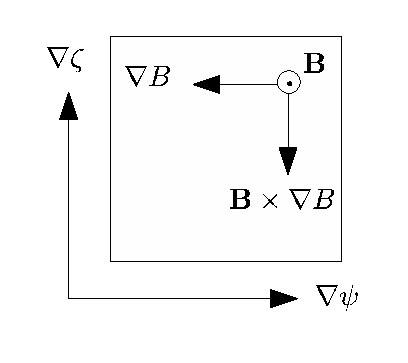
\includegraphics[width=0.3\textwidth]{directions.eps}
 \caption{\label{directions}Coordinate directions on the outboard
   plane ($s=0$) for $s_{\rm B}=1$, as output by the potential slices
   diagnostic \File{phi\#} with the coordinate labels for each point
   as output by \File{xphi} and \File{yphi} (the yphi coordinate label
   inverts the plot). For $s_{\rm B}=1$, the poloidal field is
   `upwards' ${\rm sign}(B_p \nabla \theta \cdot \nabla \zeta)= s_{\rm
     B}$. If in doubt, see Sec.~\ref{signs}.  Note that the `centre'
   of the flux tube is in the bottom left corner when output from the
   FFTs.}
 \end{center}
 \end{figure}
%This means as the matlab script mkmovie plots it.


\section{Summary: diagnostic outputs and their data format}
\label{sec.diagnos-data-format}

In GKW, most diagnostics are calculated inside the code at runtime (as
opposed to in post-processing).  The advantage of this approach is
that one does not need to store the full 5 dimensional distribution
functions at every timestep (which occupy a lot of disk space and are
difficult to transfer).  The disadvantage is that if a time dependent
diagnostic is not enabled or implemented before the run, that
information cannot later be retrieved without re-running the entire
simulation (final state diagnostics can always be retrieved by
restarting the code if the restart file is available).  One should
therefore think carefully about which diagnostics are required before
launching any expensive simulation.  One could argue that this
approach is suited to a world in which computation is cheap, but
storage and transfer are expensive.

The default set of time dependent diagnostics contains scalar time
traces (fluxes, growth rates) and 1D spectra, but no 2D or 3D
quantities.

GKW does contain a wrapper which allows to write output data
in various formats, according to the setting of \name{io_format} in
the input file.
\begin{description}
\item[\name{io_format='ascii'}] (also called 'formatted' output) All
  data is written to a collection of text files. Those can be read and
  analysed easily, and they are very portable. The ASCII format
  becomes impractical for higher dimensional and large amounts of data.

  For ascii and binary formats, diagnostic meta-data is output by the
  code to a simple text file \File{gkwdata.meta}.

\item[\name{io_format='binary'}] (also called 'raw' output) All data
  is written to binary files. Binary data consumes typically by a
  factor of about 6-10 less disk space than ascii data. Binary or hdf5
  (see below) format is therefore recommended if large amounts of data
  are produced.
\item[\name{io_format='hdf5'}] (also called 'structured' output), if
  \name{io_format='hdf5'} is set. This structured binary format is
  available if the code was compiled with the HDF5 library. If the
  HDF5 library was compiled with szip encoding support, then the GKW
  output data can be compressed (for now, there is only a hardcoded
  switch, see the comments).
  \\
%Issue 69    
  The HDF5 format allows to output diagnostic meta-data by associating
  attributes to datasets. These can be read by analysis
  scripts.  More and more metadata will be added in the near future, for
  discussions see \issue{69}. Note that
  \begin{itemize}
  \item If one tries to access HDF5 files during run, they may turn
    out to be invalid (not always though).
  \item Aborted runs may leave a corrupted HDF5 file. Usually then
    there are just no parameters in the file, sometimes datasets are
    missing and in rarer cases even the file as a whole is invalid.
  \item To produce the 3d fields and moments data and the 4d mode
    structure data, a MPI gather operation is performed and the output
    is written serially by just one process. For large runs with many
    processes this is likely not very performant. Instead, it is
    recommended to use MPI-IO binary output format then.
  \item At the time moment GKW supports only serial
    HDF5.
  \end{itemize}
\end{description}

In order to take advantage of the benefits of certain formats, GKW
knows also about mixed output:
\begin{description}
\item[\name{io_format='mixed'}] Most of the data (mainly scalar time
  traces and 1D spectra, \File{parallel.dat} final state
  eigenfunctions) is output to text files, whereas higher dimensional
  data is output to binary files.
\item[\name{io_format='hdf5+ascii'}] All data is output as with the
  'hdf5' setting. In addition, lowerdimensional data is output also to
  text files.
\end{description}

As long as there is not enough descriptive metadata attached to the
GKW diagnostic output data, we here summarize most of the GKW
diagnostic outputs in tables \ref{tab:diag-part1} and
\ref{tab:diag-part2} for 1D time traces, final state outputs, and 2D
time trace outputs.  A full listing of available diagnostics and
switches is documented in \doc{input.dat.sample}.  In the case of less
standard diagnostics it may be necessary to examine the source and
comments in the respective diagnostic module \src{diagnos_foo.F90} to
determine the exact order and meaning of the output quantities.

Generally, 2D diagnostics can be output by GKW at every timestep, or
at the end (``R or E'' in tables \ref{tab:diag-part1} and
\ref{tab:diag-part2}, switched by \name{xy_estep}). \\
When successive binary records for each timestep are stacked into one
file, this happens with (32 bit / 4 byte, usually)
integers before and after each record for the size of the binary
record (which will have Endianness of the hardware it was written on).
The data records can be
read into matlab with the script \matlab{read_file2d.m}.\\

Some slices are output at the point nearest the LFS, for
these a different location can be set with switch
\name{xy_slice_ipar}. 

\paragraph*{Reorganisation of diagnostics and the \name{io_legacy} switch:}
Note that there currently efforts to clean up GKW's diagnostics. This
includes renaming of some files, split up of datasets and change of
the order of the data, where necessary. The goal is to output data in
a more natural way which is easy to understand and to analyse.

In order to provide users for some time the possibility to keep using
their old analysis tools without larger changes, the switch
\name{io_legacy} was introduced.

\begin{landscape}
\begin{table}[hp!]
\begin{footnotesize}
\vspace{-2cm}
\begin{adjustwidth}{-1cm}{-2cm}
\centering 
\begin{tabular}{l|l|l|l|l|l|l}
 Filename / dataset name & Description & Quantity (norm.=normalised) & Size 
& when
& \parbox[t]{1cm}{Grid\\Files}
& \parbox[t]{1.5cm}{Namelist\\Switch}\\
\hline
%\File{foo} & [description] & [expression] & [rows,cols,..]  &B/R/E/O & [gridfiles] & [switch]\\
\hline\multicolumn{7}{ |c| }{\textbf{Module diagnos_growth_freq:}} \\
\File{dominant_growth_rate} & Dominant linear mode growth rate & $\gamma_{N}^{\rm max}$ & $N_t$  & R & & \\
\File{dominant_real_freq} & Dominant linear mode frequency & $\omega_N$ belonging to $\gamma_{N}^{\rm max}$& $N_t$  & R & & \\
\File{growth_rates.dat} & Growth rates of all linear modes & $\gamma_N$ &   & R & & \\
\File{frequencies.dat} & Frequencies of all linear modes & $\omega_N$ &   & R & & \\
\File{amplitudes.dat} & Amplitudes of all linear modes &  &  & R & & \\


\hline\multicolumn{7}{ |c| }{\textbf{Module diagnos_grid:}} \\
\File{time.dat} & timestamp (large time steps) & $t_N$ & $N_t$  & R & & \\
\File{sgrid} & s grid (parallel coordinate) & $s$ & $N_s$  & B & & \\
\File{krho} & Bi-normal wavevector grid & $(q / 2 \pi \psi) k_\zeta \rho_{\rm ref} = k_\perp(k_\psi=0,s=0) \rho_{\rm ref}$ & $N_x, N_{\rm mod}$& B & & \\
\File{kxrh} & Radial wavevector grid & $k_\psi \rho_{\rm ref}$ & $N_x, N_{\rm mod}$& B & & \\
\File{yphi} & Real space bi-normal grid & $ 2 \pi \psi (\zeta-\zeta_{\rm min})/q\rho_{\rm ref} = k_\theta \rho_{\rm ref}$ & $M_x,
M_{\rm mod}$ & B & & \\
\File{xphi} & Real space radial grid & $(\psi-\psi_{\rm min})/\rho_* = (r-r_{\rm min})/\rho_{\rm ref} $ & $M_x, M_{\rm mod}$ & B & & \\
\File{kx_connect} & Parallel boundary connections & Labelled in file & N/A& B & & \\
\hline\multicolumn{7}{ |c| }{\textbf{Module diagnos_mode_struct:}} \\
\File{phi} & es. potential & See Sec. \ref{sec.parallel}. & $N_{\rm MOD},  N_s, N_x$ & E and O & & \\
\File{Apar} &  & See Sec. \ref{sec.parallel}. & $N_{\rm MOD},  N_s, N_x$ & E and O & & \\
\File{Bpar} &  & See Sec. \ref{sec.parallel}. & $N_{\rm MOD},  N_s, N_x$ & E and O & & \\
\File{dens} & density fluctuations & See Sec. \ref{sec.parallel}. & $N_{\rm sp}, N_{\rm MOD},  N_s, N_x$ & E and O & & \\
\File{Tpar} & parall. temperature fluct. & See Sec. \ref{sec.parallel}. & $N_{\rm sp}, N_{\rm MOD},  N_s, N_x$ & E and O & & \\
\File{Tperp} & perp. temp. fluctuations & See Sec. \ref{sec.parallel}. & $N_{\rm sp}, N_{\rm MOD},  N_s, N_x$ & E and O & & \\
\File{vpar} & parallel flow fluctuations & See Sec. \ref{sec.parallel}. & $N_{\rm sp}, N_{\rm MOD},  N_s, N_x$ & E and O & & \\

\hline\multicolumn{7}{ |c| }{\textbf{Module diagnos_fields:}} \\
\File{kyspec} & Bi-normal mode potential spectrum &  $\sum_{k_\psi} \int_{s} |\hat \phi(k_\psi,k_\zeta,s)|^2 \, {\rm d}s $    &  $N_t,N_{\rm mod}$& R & & \\
\File{kyspec_em} & (Equivalent for $A_\parallel$ field) & $\sum_{k_\psi} \int_{s} |\hat A_\parallel(k_\psi,k_\zeta,s)|^2 \, {\rm d}s $ & $N_t,N_{\rm mod}$ & R\\
\File{kxspec(_em)} & Radial mode potential spectrum &  $\sum_{k_\zeta} \int_{s} |\hat \phi(k_\psi,k_\zeta,s)|^2 {\rm d}s $  & $N_t,N_x$  & R & & \\
\File{kyvort} & Bi-normal vorticity spectra &  $\sum_{k_\psi,sp} \int Z_{sp}|\hat f_{sp}(k_\psi,k_\zeta,s)|^2 \, {\rm d}^3 v \, {\rm d}s $  & $N_t,N_{\rm mod}$ & R & & \\

\File{kxvort} & Radial vorticity spectra &  $\sum_{k_\zeta,sp} \int Z_{sp} |\hat f_{sp}(k_\psi,k_\zeta,s)|^2 \, {\rm d}^3 v \, {\rm d}s $  & $N_t,N_x$ & R & & \\
\hline
\File{spc\#}  & ES potential spectrum (LFS) & $|\hat \phi(k_\psi,k_\zeta,s\approx0)|$ \ (norm.)& &R or E & \File{kxrh, krho} & \name{xy_phi} \\

\File{phi\#}  & ES potential slice (LFS) &  $\phi(\psi,\zeta,s\approx0)$ \ (norm.)&  &R or E & \File{xphi, yphi} & \name{xy_phi} \\

\File{apc\#}  & EM potential spectrum (LFS) &   $|\hat A_\parallel (k_\psi,k_\zeta,s\approx0)|$ \ (norm.)& &R or E & \File{kxrh, krho} & \name{xy_apar} \\

\File{apa\#}  & EM potential slice (LFS) &  $A_\parallel(\psi,\zeta,s\approx0)$\ (norm.) & &R or E & \File{xphi, yphi} & \name{xy_apar} \\

\File{bpc\#}  & EM field spectrum (LFS) &  $|\hat B_\parallel(k_\psi,k_\zeta,s\approx0)|$ \ (norm.)& &R or E & \File{kxrh, krho} & \name{xy_bpar} \\

\File{bpa\#}  & EM field slice (LFS) &  $B_\parallel(\psi,\zeta,s\approx0)$ \ (norm.)& &R or E & \File{xphi, yphi} & \name{xy_bpar} \\

\File{vok\#}  & Vorticity spectrum (FSA) &  $\sum_{s} \int |\hat f_{s}(k_\psi,k_\zeta)| d^3 v ds$ \ (norm.)& &R or E & \File{kxrh, krho} & \name{xy_vort}\\


\hline\multicolumn{7}{ |c| }{\textbf{Module diagnos_moments:}} \\
\File{ene[sp\#]_\#}  & Temp. pert. moment (LFS) &  $\sum_{sp} \int |\hat f_{s} v^2| d^3 v $ \ (norm.)& &R or E & \File{xphi, yphi} & \name{xy_temp} \\

\File{den[sp\#]_\#}  & Density pert. moment (LFS) &  $\int |\hat f_{s}| d^3 v $ \ (norm.)& &R or E & \File{xphi, yphi} & \name{xy_dens} \\

\File{pac[sp\#]_\#}  & Current pert. moment (LFS) &  $\int |\hat f_{s} | v_\parallel d^3 v $ \ (norm.)& &R or E & \File{xphi, yphi} & \name{xy_current} \\

\File{pac[sp\#]_\#}  & Current$^2$ pert. moment (LFS) &  $\int |\hat f_{s} | v_\parallel^2 d^3 v $ \ (norm.) & &R or E & \File{xphi, yphi} & \name{xy_current2} \\

\File{{den/ene}_spectra} & \parbox[t]{3.5cm}{Bi-normal spectral perturbation moments for each species} & $\sum_{k_\psi}\int_s \int \hat \alpha_{1,2} |\hat f_{sp}| {\rm d}^3v \, {\rm d}s $ & $N_{\rm mod},N_{sp}$ & & & \\

\end{tabular}
\end{adjustwidth}
\end{footnotesize}
\caption{
  Diagnostics output by GKW (Part 1), with \name{io_legacy=false}. The
  abbreviations denote output at the beginning (B), repeatedly (R), at the end
  (E) or other (O). FSA denotes Flux Surface Averaged quantities. LFS denotes quantities evaluated at the low field side, i.e. in the center of the $s$-grid.
}
\label{tab:diag-part1}
\end{table}
\end{landscape}

\begin{landscape}
\begin{table}[hp!]
\begin{footnotesize}
\vspace{-2cm}
\begin{adjustwidth}{-1cm}{-1cm}
\centering 
\begin{tabular}{l|l|l|l|l|l|l}
 Filename / dataset name & Description & Quantity (norm.=normalised) & Size 
& \parbox[t]{2cm}{beginning (B),\\ repeatedly (R),\\ at the end (E)}
& \parbox[t]{1cm}{Grid\\Files}
& \parbox[t]{1.5cm}{Namelist\\Switch}\\
\hline
\hline\multicolumn{7}{ |c| }{\textbf{Module diagnos_moments:}} \\
\File{dens_kyzero_xs[sp\#]_\#}    & Density pert. moment ($k_\zeta = 0$) &  $\int |\hat f_{sp}| d^3 v $ \ (norm.)            & &R  & \File{xphi, sgrid} & \name{xs_kyzero_dens} \\
\File{current_kyzero_xs[sp\#]_\#} & Current pert. moment ($k_\zeta = 0$) &  $\int |\hat f_{sp}| v_\parallel d^3 v $ \ (norm.)& &R  & \File{xphi, sgrid} & \name{xs_kyzero_current} \\
\File{ene_kyzero_xs[sp\#]_\#}     & Energy pert. moment ($k_\zeta = 0$)  &  $\int |\hat f_{sp}| v^2 d^3 v $ \ (norm.)& &R  & \File{xphi, sgrid} & \name{xs_kyzero_ene} \\
\File{ene_par_kyzero_xs[sp\#]_\#}     & Parallel energy pert. moment ($k_\zeta = 0$)  &  $\int |\hat f_{sp}| v_\parallel^2 d^3 v $ \ (norm.)& &R  & \File{xphi, sgrid} & \name{xs_kyzero_ene_par} \\
\File{ene_perp_kyzero_xs[sp\#]_\#}     & Perpendicular energy pert. moment ($k_\zeta = 0$)  &  $\int |\hat f_{sp}| v_\perp^2 d^3 v $ \ (norm.)& &R  & \File{xphi, sgrid} & \name{xs_kyzero_ene_perp} \\
\File{phi_ga_fm_kyzero_xs[sp\#]_\#}     & Gyro-averaged (using $F_M$) el.-stat. potential  ($k_\zeta = 0$)  &  $\int |\hat F_{M,sp}| \langle \hat \phi \rangle d^3 v $ \ (norm.)& &R  & \File{xphi, sgrid} & \name{xs_kyzero_phi_ga_fm} \\

\hline\multicolumn{7}{ |c| }{\textbf{Module diagnos_fluxes:}} \\
%\File{fluxes.dat} & Total $v_E$ fluxes $(i=1,2,3)$ by species  & ${\cal I}_i=\sum_{k_\zeta} \sum_{k_\psi} \int_{s} \bar{\cal I}_i \, {\rm d}s$  & $3N_{sp}$ & R & & \\
\File{p/e/vflux_es} & Total $v_E$ particle/heat/momentum flux by species  & ${\cal I}_i=\sum_{k_\zeta} \sum_{k_\psi} \int_{s} \bar{\cal I}_i \, {\rm d}s$  & $N_t,N_{sp}$ & R & \File{time} & \\
\File{p/e/vflux_es_lab} & Corresponding Lab frame fluxes & ${\cal I}_i+d{\cal I}_i$  & $N_t,N_{sp}$ & R & \File{time} & \\
%\File{eflux_es} & Total $v_E$ heat flux by species  & ${\cal I}_2=\sum_{k_\zeta} \sum_{k_\psi} \int_{s} \bar{\cal I}_2 \, {\rm d}s$  & $N_t,N_{sp}$ & R & \File{time} & \\
%\File{vflux_es} & Total $v_E$ momentum flux by species  & ${\cal I}_3=\sum_{k_\zeta} \sum_{k_\psi} \int_{s} \bar{\cal I}_3 \, {\rm d}s$  & $N_t,N_{sp}$ & R & \File{time} & \\
\File{p/e/vflux_apar} & Total $A_\parallel$ particle/heat/momentum flux by species  & ${\cal J}_i=\sum_{k_\zeta} \sum_{k_\psi} \int_{s} \bar{\cal J}_i \, {\rm d}s$  & $N_t,N_{sp}$ & R &  \File{time} & \\
\File{p/e/vflux_apar_lab} &  Corresponding Lab frame fluxes & ${\cal J}_i+d{\cal J}_i$  & $N_t,N_{sp}$ & R &  \File{time} & \\
%\File{eflux_apar} & Total $A_\parallel$ heat flux by species  & ${\cal J}_2=\sum_{k_\zeta} \sum_{k_\psi} \int_{s} \bar{\cal J}_2 \, {\rm d}s$  & $N_t,N_{sp}$ & R &  \File{time} & \\
%\File{vflux_apar} & Total $A_\parallel$ momentum flux by species  & ${\cal J}_3=\sum_{k_\zeta} \sum_{k_\psi} \int_{s} \bar{\cal J}_3 \, {\rm d}s$  & $N_t,N_{sp}$ & R &  \File{time} & \\
\File{p/e/vflux_bpar} & Total $\nabla B_\parallel$ particle/heat/momentum flux by species  & ${\cal K}_i=\sum_{k_\zeta} \sum_{k_\psi} \int_{s} \bar{\cal K}_i \, {\rm d}s$  & $N_t,N_{sp}$ & R &  \File{time} & \\
\File{p/e/vflux_bpar_lab} & Corresponding Lab frame fluxes  & ${\cal K}_i + d{\cal K}_i$  & $N_t,N_{sp}$ & R &  \File{time} & \\
%\File{eflux_bpar} & Total $\nabla B_\parallel$ heat flux by species  & ${\cal K}_2=\sum_{k_\zeta} \sum_{k_\psi} \int_{s} \bar{\cal K}_2 \, {\rm d}s$  & $N_t,N_{sp}$ & R &  \File{time} & \\
%\File{vflux_bpar} & Total $\nabla B_\parallel$ momentum flux by species  & ${\cal K}_3=\sum_{k_\zeta} \sum_{k_\psi} \int_{s} \bar{\cal K}_3 \, {\rm d}s$  & $N_t,N_{sp}$ & R &  \File{time} & \\

\File{{p/e/v}flux_spectra} & Bi-normal spectral $v_E$ flux for each species & $\sum_{k_\psi} \int_{s} \bar {\cal I}_i(k_\psi,k_\zeta) \, {\rm d}s$ & $N_t,N_{\rm mod},N_{sp}$ & R & & \\

\File{{p/e/v}flux_xspec}  & Radial spectral $v_E$ fluxes for each species & $\sum_{k_\zeta} \int_{s} \bar {\cal I}_i(k_\psi,k_\zeta) \, {\rm d}s$  & $N_t,N_{\rm mod},N_{sp}$   & R & & \\

\File{{p/e}flux_(em_)sup} & \parbox[t]{3.5cm}{Bi-normal spectral flux suprema for each species} & $\hat {\cal I}_i(k_\zeta), \hat {\cal J}_i(k_\zeta) $ & $N_t,N_{\rm mod},N_{sp}$ & R & & \\

\hline
\File{PFlesr[sp\#]_\#}  & ES radial particle flux (LFS) & ${\cal I}_1(\psi,\zeta,s\approx0)$\ (norm.)& & R or E & \File{xphi, yphi} & \name{xy_fluxes_P} \\

\File{EFlesr[sp\#]_\#}  & ES radial energy flux (LFS) & ${\cal I}_2(\psi,\zeta,s\approx0)$ \ (norm.)& & R or E & \File{xphi, yphi} & \name{xy_fluxes} \\

\File{VFlesr[sp\#]_\#}  & ES radial momentum flux (LFS) & ${\cal I}_3(\psi,\zeta,s\approx0)$ \ (norm.)& & R or E & \File{xphi, yphi} & \name{xy_fluxes_V} \\

\File{[P/E/V]Fl\underline{em}r[sp\#]_\#}  & EM flutter fluxes as above (LFS) &  $J_i(\psi,\zeta,s\approx0)$ \ (norm.) & & R or E & \File{xphi, yphi} & \name{+ xy_fluxes_em} \\

\File{[P/E/V]Fl\underline{bp}r[sp\#]_\#}  & EM comp. fluxes as above (LFS) &  $K_i(\psi,\zeta,s\approx0)$ \ (norm.)& & R or E & \File{xphi, yphi} & \name{+ xy_fluxes_bpar} \\

\File{[P/E/V]F\underline{S}[es/em/bp]r[sp\#]_\#}  & All fluxes as abv., but (FSA) &  $\int I_i/J_i/K_i(\psi,\zeta) ds$ \ (norm.)& & R or E & \File{xphi, yphi} & \name{+ xy_fluxes_fsa} \\

\File{[P/E/V]F[l/S][es/em/bp]\underline{p}[sp\#]_\#}  & Binormal fluxes as abv. (LFS/FSA)&  N/A & & R or E & \File{xphi, yphi} & \name{+ xy_fluxes_bi} \\

\File{[P/E/V]Fl[es/em/bp]\underline{k}[sp\#]_\#}  & Radial fluxes spectra (FSA) &  $\int I_i/J_i/K_i(k_\psi,k_\zeta) ds$ \ (norm.)& & R or E & \File{kxrh, krho} &  \name{+ xy_fluxes_k} \\

\hline\multicolumn{7}{ |c| }{\textbf{Module diagnos_fluxes_vspace:}} \\
\File{fluxes_det.dat} & \parbox[t]{4cm}{5D fluxes for each species, \\including $\ud^3X$ and $\ud^3v$}& $\Big(\bar{\cal I}_i + \bar{\cal J}_i +  \bar{\cal K}_i\Big)(k_\psi,k_\zeta,s,\mu,v_\parallel)$  & \parbox[t]{2cm}{binary, $N_{v_\parallel} N_\mu N_s\\ N_\psi N_{mod} N_{sp} i,$\\$i=1,2,3$}& E & & \name{lfluxes_detail} \\
\hline

\File{[p/e/v]fluxes_vspace[sp\#]_\#}  & Fluxes in velocity space (FSA) &  $\int I_i/J_i/K_i(v_\parallel,\mu) ds$ \ (norm.)& &R or E & \File{distr[1/2]} & \name{lfluxes_vspace} \\

%\hline\multicolumn{7}{ |c| }{\textbf{Module diagnos_rad:}} \\
%\hline\multicolumn{7}{ |c| }{\textbf{Module diagnos_velspace:}} \\
%\hline\multicolumn{7}{ |c| }{\textbf{Module diagnos_energetics:}} \\
\hline\multicolumn{7}{ |c| }{\textbf{Module diagnos_f:}} \\
\File{distr*.dat}   & 2D velocity space output of 1 mode. & 1,2 grids, 3 Re$({\hat g}(s=0))$, 4 Im$({\hat g}(s=0))$ & $N_\mu$, $N_{v_\parallel}$ & E & & \\
%\hline\multicolumn{7}{ |c| }{\textbf{Module diagnos_stresses:}} \\
%\hline\multicolumn{7}{ |c| }{\textbf{Module diagnos_zfshear:}} \\
%\hline\multicolumn{7}{ |c| }{\textbf{Module diagnos_eng:}} \\
%\hline\multicolumn{7}{ |c| }{\textbf{Module diagnos_nonlin_transfer:}} \\

\hline\multicolumn{7}{ |c| }{\textbf{Output by other parts of the code:}} \\
\File{parfun.dat} & Perpendicular wavevector & $k_\perp\rho_{\rm ref}$ & $2,N_s N_{\rm mod} N_x$& B & & \\
\File{par.dat} & Curvature and Coriolis functions & $k_\perp\rho_{\rm ref}$ , ${\cal D}^\psi k_\psi + {\cal
D}^\zeta k_\zeta$, ${\cal H}^\psi k_\psi + {\cal H}^\zeta k_\zeta$, & $3,N_s N_{\rm mod} N_x$& B & & \\
\File{geom.dat} & Geometry tensors & Labelled in file & N/A& B & & \\
\File{FDS}        & Restart distribution function  & binary (see Sec. \ref{sec.restart})& E & & \\
\File{FDS.dat}    & Additional restart information & Ascii namelists (see Sec. \ref{sec.restart}) & E & & \\
\File{Coll_params.dat} & Collision frequencies & Labelled in file & N/A & B & & \\
\File{cfdens.dat} & Centrifugal poloidal density variations & $s$, $R/L_{\rm n, sp}^E(s)$, $exp(-\cfenn)_{\rm sp}(s), \theta$ &  $2 N_{\rm sp} + 2$ & B & & \\
\end{tabular}
\end{adjustwidth}
\end{footnotesize}
\caption{
  Diagnostics output by GKW (Part 2) , with \name{io_legacy=false}.
}
\label{tab:diag-part2}
\end{table}
\end{landscape}

\begin{landscape}
\begin{table}[hp!]
\begin{footnotesize}
\vspace{-2cm}
\begin{adjustwidth}{-1cm}{-2cm}
\centering 
\begin{tabular}{l|l|l|l|l|l|l}
 Filename & Description & Quantity (norm.=normalised) & Cols,(Rows) 
& \parbox[t]{2cm}{beginning (B),\\ repeatedly (R),\\ at the end (E)}
& \parbox[t]{1cm}{Grid\\Files}
& \parbox[t]{1.5cm}{Namelist\\Switch}\\
\hline
\hline\multicolumn{7}{ |c| }{\textbf{Module diagnos_growth_freq:}} \\
\File{time.dat} & Dominant linear mode growth rate & $t_N, \gamma_{N}^{\rm max}, \omega_N$ & 3  & R & & \\
\File{growth.dat} & Growth rates of all linear modes & $\gamma_N$ &   & R & & \\
\hline\multicolumn{7}{ |c| }{\textbf{Module diagnos_mode_struct:}} \\
\File{parallel.dat} & Parallel mode structure & See Sec. \ref{sec.parallel}. & $N_{\rm MOD} N_x N_s N_{\rm sp}$ & E & & \\
\hline\multicolumn{7}{ |c| }{\textbf{Module diagnos_moments:}} \\
\File{{den/ene}_spectra} & \parbox[t]{3.5cm}{Bi-normal spectral perturbation  moments for each species} & $\sum_{k_\psi}\int_s \int \hat \alpha_{1,2} |\hat f_{sp}| {\rm d}^3v \, {\rm d}s $ & $N_{\rm mod}N_{sp}$ & & & \\
\hline\multicolumn{7}{ |c| }{\textbf{Module diagnos_fluxes:}} \\
\File{fluxes.dat} & Total $v_E$ fluxes $(i=1,2,3)$ by species  & ${\cal I}_i=\sum_{k_\zeta} \sum_{k_\psi} \int_{s} \bar{\cal I}_i \, {\rm d}s$  & $3N_{sp}$ & R & & \\
\File{fluxes_lab.dat} & Total Lab frame $v_E$ fluxes $(i=1,2,3)$ by species  & ${\cal I}_i + d{\cal I}_i$  & $3N_{sp}$ & R & & \\
\File{fluxes_em.dat} & Total $\delta B$ fluxes $(i=1,2,3)$ by species  & ${\cal J}_i=\sum_{k_\zeta} \sum_{k_\psi} \int_{s} \bar{\cal J}_i \, {\rm d}s$  & $3N_{sp}$ & R & & \\
\File{fluxes_em_lab.dat} & Total Lab frame $\delta B$ fluxes $(i=1,2,3)$ by species  & ${\cal J}_i+d{\cal J}_i$  & $3N_{sp}$ & R & & \\
\File{fluxes_bpar.dat} & Total $\nabla B_{1 \parallel}$ fluxes $(i=1,2,3)$ by species  & ${\cal K}_i=\sum_{k_\zeta} \sum_{k_\psi} \int_{s} \bar{\cal K}_i \, {\rm d}s$  & $3N_{sp}$ & R & & \\
\File{fluxes_bpar_lab.dat} & Total Lab frame $\nabla B_{1 \parallel}$ fluxes $(i=1,2,3)$ by species  & ${\cal K}_i+d{\cal K}_i$  & $3N_{sp}$ & R & & \\
\end{tabular}
\end{adjustwidth}
\end{footnotesize}
\caption{
  Legacy diagnostics output by GKW, with \name{io_legacy=true}. This table shows
  output datasets which differ from the ones described in
  tables \ref{tab:diag-part1} and \ref{tab:diag-part2} which
  are associated with \name{io_legacy=false}.
}
\label{tab:diag-legacy}
\end{table}

\end{landscape}

\newpage
 
\section{Island torque and stabilization by the parallel current}

A diagnostic especially useful for tearing mode dynamics is the one giving the torque and the stabilization
 by the parallel current, namely $T_\varphi$ and $\Delta_{\rm pol}$, respectively. These quantities are defined as follows, under
the assumption of a non rotating island
\begin{equation}
T_\varphi \propto \int_{-L_x/2}^{L_x/2}\, dx\, \int_{-\pi}^{\pi}\, d\zeta_0\,\,J_\parallel\sin\left(\kappa_{\zeta,\rm isl}\zeta_0\right)
\label{torque}
\end{equation}
\begin{equation}
\Delta_{\rm pol} \propto \int_{-L_x/2}^{L_x/2}\, dx\, \int_{-\pi}^{\pi}\, d\zeta_0\,\,J_\parallel\cos\left(\kappa_{\zeta,\rm isl}\zeta_0\right)
\label{deltaprime}
\end{equation}
where $L_x$ is the width of the simulation box in the radial direction, the variable $\zeta_0$ is the
helical co-ordinate in the absence of rotation and $J_\parallel$ is the gyro-centre parallel
current, given by
\begin{equation}
J_\parallel = \sum_{s}eZ_s\int_{\mathbb{R}^3} \, d^3\mathbf{v}\, v_\parallel \delta f_s
\end{equation}
with $\delta f_s$ the perturbed distribution function of the gyro-centres of species $s$.
Note that multiplying equation \ref{torque} by $-i$
and adding the resulting expression to equation \ref{deltaprime} yields
\begin{equation}
\Delta_{\rm pol} - i T_\varphi \propto \sum_{s}eZ_s\int_{-L_x/2}^{L_x/2}\, dx\, \int_{-\pi}^{\pi}\, d\zeta_0\, \int_{\mathbb{R}^3} \, d^3\mathbf{v} \, v_\parallel \delta f_s\, \exp\left(-i\kappa_{\zeta,\rm isl}\zeta_0\right)
\end{equation}
where we can distinguish the Fourier mode $\hat{\delta f_s}_{isl}\equiv\hat{\delta
f_s}\left(\kappa_\zeta=\kappa_{\zeta,\rm isl}\right)\propto\int_{-\pi}^{\pi}\, d\zeta_0\, \delta f_s \, \exp\left(-i\kappa_{\zeta,\rm isl}\zeta_0\right)$, with $\kappa_{\zeta,\rm isl}$ being the mode
 of the island in the binormal direction. Therefore, we can write
\begin{equation}
\Delta_{\rm pol} - i T_\varphi \propto \sum_{s}eZ_s\int_{-L_x/2}^{L_x/2}\, dx\, \int_{\mathbb{R}^3} \, d^3\mathbf{v} \, v_\parallel \hat{\delta f_s}_{\rm isl}
\end{equation}
A rotating island is usually imposed or obtained self-consistently in GKW. This means that the island is not
 always in the middle of the simulation box in the binormal direction. However, the above expressions are
 obtained assuming that the island is centered and therefore need to be corrected by multiplying
 by the phase $\exp\left(i\int_0^t \,dt' \omega_{\rm isl}\right)$, where $\omega_{\rm isl}$ is the rotation of the island, which results
 in the definition of the co-ordinate $\zeta = \zeta_0 - \int_0^t\, dt'\omega_{\rm isl}$. Note that in the absence
 of rotation, the amplitude of the vector potential $A_\parallel$ is real, due to the fact that a pure
 $\cos\left(\kappa_\zeta \zeta\right)$ is represented in GKW by a real amplitude of $A_\parallel$. Therefore,
 any departure from a real amplitude in $A_\parallel$ implies a rotation $\omega_{\rm isl}$, which can be calculated as
\begin{equation}
\int_0^t \, dt' \omega_{\rm isl} = \arctan\left(\frac{\Im\left(A_\parallel\right)}{\Re\left(A_\parallel\right)}\right)
\end{equation}
leading to the expression
\begin{equation}
\mathcal{T}\equiv\Delta_{\rm pol} - i T_\varphi \propto \sum_{s}eZ_s\int_{-L_x/2}^{L_x/2}\, dx\, \int_{\mathbb{R}^3} \, d^3\mathbf{v} \, v_\parallel \hat{\delta f_s}_{\rm isl}\exp\left(i\int_0^t \, dt' \omega_{\rm isl}\right)
\end{equation}

Finally, the torque and instability parameter are calculated as
\begin{equation}
T_\varphi = -\Im\left(\mathcal{T}\right)
\end{equation}
\begin{equation}
\Delta_{\rm pol} = \Re\left(\mathcal{T}\right)
\end{equation}

These two quantities are output in the files \File{torque.dat} and \File{deltaprime.dat}, respectively. The first column corresponds to
 the values for the ions and the second column to the values for the electrons.

\pagebreak

\section{Entropy (module \texttt{diagnos\_energetics} and \texttt{diagnos\_eng})}

% To cite ?
% Candy PoP 13, 032310 (2006):  Does this not relate directly to what we have ?
% Krommes 94

\subsection{Definition of the Total Entropy of the Simulated Box}\label{sec:entr-simul-box}
Let $p(\mathbf{X},v_\parallel, \mu) \in [0,1]$ be a probability density function.

One can define the functional
\begin{equation}
  \label{eq:bgs-entropy}
  S = -\int\!\ud^3x\ud^3v p\ln(p\cdot c_d),\qquad c_d = \mathrm{const.}
\end{equation}
and show that this expression has properties of the thermodynamical entropy (see e.g.\ the book of Jelitto 1989). It is therefore called ``statistical entropy'' or Shannon-Jaynes-entropy or Pauli-entropy or Boltzmann-Shannon-Gibbs (BGS) entropy. 
 A constant $c_d$ is formally needed in \ref{eq:bgs-entropy} to make the logarithm dimensionless \cite{DUN07} but it can be set equal to 1. Note that the integral in \ref{eq:bgs-entropy} is over the whole system, i.e.\ derived integrals below, on quantities of the simulated model, are taken over the whole simulation box. 

A ``relative entropy'' functional can be defined in the form
\begin{equation}
  \label{eq:relative-entropy}
  S = -\int\!\ud^3x\ud^3v\ p\ln \frac{p}{q}
\end{equation}
This functional characterizes the distribution $p$ with respect to a certain reference probability density function $q \in [0,1]$ . 


Maximization of the relative entropy $S$ under the constraint
\begin{align}\label{eq:maximizationSconstraint}
  1 = \int\ud\mathbf{x}\ud\mathbf{v}\,p(\mathbf{x},\mathbf{v})
\end{align}
leads to the condition
\begin{align}
  0 = 1 + ln\frac{p}{q} + \alpha
\end{align}
and thus
\begin{align}\label{eq:maximizationSp}
  p = q\cdot\exp[-(1+\alpha)]\
\end{align}
the distribution which corresponds to the extremum of the functional depends on the reference. With the assumption that the reference PDF $q$ fulfills
\ref{eq:maximizationSconstraint}, one applies this constraint \ref{eq:maximizationSconstraint} to \ref{eq:maximizationSp} and finds then $\alpha = -1$ and so
\begin{align}
  p = q ,
\end{align}
that means the entropy has its extremum for $p=q$.
Variation of the relative entropy under other constraints, using a reference which fulfills those, leads to the condition $p = q$ by the same argument.

% Is it not the neoclassical canoncial Maxwellian that is really the maximum entropy distribution ?
For a PDF describing an ensemble of classical particles, the distribution which maximizes the entropy under two contraints (normalisation of the distribution and given kinetic energy average) is the Maxwellian. 
For our purposes, we put therefore $f_{tot}$ in place of $p$ and the reference
distribution is chosen to be the Maxwell distribution in velocity space and to
describe particle trapping (and possibly centrifugal trapping) in position space.
This Maxwellian distribution function is denoted with $F_M$ and is given in equation \eqref{eq:maxwell}.
\begin{equation}
  \label{eq:relative-entropy-with-f}
  S = -\int\!\ud^3X\ud^3v f_{tot}\ln \frac{f_{tot}}{F_M}
\end{equation}
A state of maximum entropy then corresponds to $f_{tot} = F_M$. In the $\delta f$ model, where the distribution is split into $f_{tot} = F_M + f$, this means that the distribution perturbation vanishes in the thermodynamic equilibrium: $f = 0$.

Furthermore, it can be shown \cite{DUN07} that in contrast to the BGS entropy \ref{eq:bgs-entropy} given first, maximizing the relative entropy \ref{eq:relative-entropy} leads to the same distribution function, independently of the coordinate system. This is an important property if we want to investigate systems relaxing towards equilibrium in the field aligned coordinate system in which the gyrokinetic model is formulated. The invariance under coordinate transformations of the maximum-entropy principle associated with the relative entropy notion \ref{eq:relative-entropy} guarantees that the distribution $f_{tot} = F_M$ really corresponds to the maximum value of the entropy, and not another distribution, e.g.\ by multiplication with a factor.

Reduction of the perturbation $|f|$ means growth of the entropy $S$, i.e.\ the system moves towards thermodynamic equilibrium. On the contrary, processes that grow fluctuations $|f|$ effectively diminish the entropy of the system and keep it away from equilibrium, which is by definition the macrostate of maximum entropy.

We set $f_{tot} = F_M + f$ and expand around $f=0$: 
\begin{align}
  (F_M + f)\ln\frac{F_M + f}{F_M} &= (F_M + f)\left[0 + \frac{1}{F_M + f}|_{f=0}f^1 + \frac{1}{2}\frac{-1}{(F_M + f)^2}|_{f=0}f^2 + \ldots\right] \nonumber\\
  &= 0 + f + \frac{f^2}{F_M} - \frac{1}{2}\frac{f^2}{F_M} + \ldots \nonumber\\
  &= 0 + f + \frac{1}{2}\frac{f^2}{F_M} + \ldots
                     % \ln\frac{F_M + f}{F_M} &=  0 + \frac{f}{F_M} - \frac{1}{2}\frac{f^2}{F_M^2}\ldots + \ldots
\end{align}
Then \ref{eq:relative-entropy-with-f} becomes
\begin{align}
  \label{eq:def-entropy}
  S \approx -\int\!\ud^3X\ud^3v (f + \frac{1}{2}\frac{f^2}{F_M}) = -\frac{1}{2}\int\!\ud^3X\ud^3v\frac{f^2}{F_M}
\end{align}
where the integral of the fluctuation $f$ vanishes. 
$S$ in \ref{eq:def-entropy} is a small-amplitude approximation to the plasma entropy.  % \cite{krommes94}
 Again, one can see that reduction of $|f|$ means increase of the entropy $S$.

In its normalized form  \ref{eq:def-entropy} is 
\begin{equation}
  \label{eq:entropy}
  S \approx -\frac{1}{2}\int\!\ud^3X\ud^3v\frac{f^2}{F_M} = \rho_*^2 \frac{v_{thref}}{R_{ref}}n_{R_0}\underbrace{\left(-\frac{1}{2}\int\!\ud^3X\ud^3v_N\frac{f_N^2}{F_{MN}}\right)}_{S_N}
\end{equation}
In the normalized balance equation \ref{eq:entropy-balance} the reference quantities are dropped, but the smallness parameter $\rho_*$ is kept for illustration.

The quantity $H = -S$ is a measure of the intensity of the fluctuations in the distribution.% \cite{candywaltz06}
\begin{equation}
  \label{eq:intensity}
  H \approx \frac{1}{2}\int\!\ud^3X\ud^3v\frac{f^2}{F_M} = \rho_*^2 \frac{v_{thref}}{R_{ref}}n_{R_0}\underbrace{\left(\frac{1}{2}\int\!\ud^3X\ud^3v_N\frac{f_N^2}{F_{MN}}\right)}_{H_N}
\end{equation}
%Being a positive functional of the distribution, the intensity $H$ is an energy-like quantity \cite{krommes94}.
%FIXME This may be interesting when looking at the growth of unstable fluctuations? \cite{krommes94}

To emphasise, the fluctuation intensity $H$ is found to be \emph{increasing} in the simulations of a system driven out of equilibrium by applied thermodynamic forces (temperature and density gradient). Accordingly the entropy $S=-H$ is found to decrease.

\subsection{Entropy Balance\label{sec:entr-balance}}

\subsubsection*{General procedure} 
One starts from the normalized gyrokinetic equation given in section \ref{equations}, multiplies every term with $\frac{f}{F_M}$ and integrates over the box volume and velocity space.

In this section, all quantities are normalized, but we omit the index $N$ here. Moreover, only the electrostatic case is considered, so that $g = f$ for the purposes of this section.

\begin{align}\label{eq:entropy-balance}  
\rho_*^2\int\!\ud^3X\ud^3v\frac{f}{F_M}\Big[\pd{g}{t} +\mathrm{I} + \mathrm{II} + \mathrm{III} + \mathrm{IV} + \mathrm{V} + \mathrm{VI} + \mathrm{VII} + \mathrm{VIII}\Big] = 0 
\end{align}

\subsubsection*{Regard the terms separately}
One can recover $\pd{\ }{t} H$ in the very first integral.
\begin{align}
  \label{eq:dSdt}
  \rho_*^2\int\!\ud^3X\ud^3v\frac{f}{F_M}\pd{g}{t} &= \rho_*^2\int\!\ud^3X\ud^3v\frac{1}{F_M}\frac{1}{2}\pd{f^2}{t} \nonumber\\
&= \pd{H}{t} = - \pd{S}{t}
\end{align}

The linear $\mathbf{E}\times\mathbf{B}$-drift term V yields
\begin{align} 
  \rho_*^2\int\!\ud^3X\ud^3v\frac{f}{F_M}\ \mathrm{V} & = \rho_*^3\int\!\ud^3X \Bigg[-\frac{1}{L_n}\Gamma_N^\psi - Q_N^\psi\frac{1}{L_T}\nonumber\\
  &\quad +\frac{3}{2}\frac{1}{L_T}\Gamma^\psi - \frac{\mathcal{E}_R}{T_R}\frac{1}{L_T}\Gamma^\psi +\nonumber\\
  &\quad - \frac{2}{T_R}\Pi_\varphi^\psi u^\prime
  - 2\frac{m_R}{T_R}\Omega_N^2\mathcal{L}\,\Gamma^\psi \Bigg]
\end{align}
At the moment these six terms are output separately by the code, but
very likely they will be combined in the near future to fewer, more
symmetric quantities.

The Landau-Damping terms VI and VII give non-vanishing contributions,
too. In combination with the Poisson equation, they can be
rewritten as
\begin{align}
  \rho_*^2\int\!\ud^3X\ud^3v\frac{f}{F_M}\Big[\mathrm{VII} + \mathrm{VIII}\Big] &= \int\ud^3X \pd{}{t} \sum_s\int\ud^3v \frac{Z_s^2}{2T_s^2}F_M\left(\phi^2(\mathbf{x}) - \Ga{\phi}^2 \right) \\
 \text{and $W_s$ is defined such that} &= \pd{}{t}\sum_sW_s \\
 W_{N,s} = {}& \int\ud^3X_N \int\ud^3v_N \frac{Z_s^2}{2T_{R,s}^2}F_{MN}\left(\phi_N^2 -  \Ga{\phi_N}^2\right)   \label{eq:W}
\end{align}
If only ion dynamics is simulated and electrons are treated
adiabatically, the index $s$ above only runs over ion species and the
term $W_{N,e}$ for the electrons is different.
\begin{align}
\pd{}{t}W_{N,e,adia}
{}={}& \pd{}{t}\int\ud^3X_N \phi_N \int\ud^3v_N\frac{Z_e}{T_{R,e}}\iGa{f_{eN}} \nonumber\\
{}={}& \pd{}{t}\int\ud^3X_N \phi_N \frac{Z_e}{T_{R,e}}n_R\frac{Z_e}{T_{R,e}}\left(\phi_N - \fsa{\phi_N} \right) \nonumber\\
{}={}& \int\ud^3X_N  n_R\frac{Z_e^2}{2T_{R,e}^2}\left(
 \pd{\phi_N^2}{t} - 2\phi_N\pd{}{t}\fsa{\phi_N}
 \right)
\end{align}
And with $\fsa{.}=\fsa{.}(\psi,\zeta)$ and $T_{R,e}^2$ being constant
with respect to the parallel direction, one can write
\begin{align}
{}={}& \int\ud\psi\ud\zeta J_X   n_R\frac{Z_e^2}{2T_{R,e}^2}\left(
\pd{\fsa{\phi_N^2}}{t} -
 2\fsa{\phi_N}\pd{}{t}\fsa{\phi_N}
 \right)\\
{}={}& \int\ud\psi\ud\zeta J_X   n_R\frac{Z_e^2}{2T_{R,e}^2}\left(
 \pd{\fsa{\phi_N^2}}{t} -
\pd{\fsa{\phi_N}^2}{t}
  \right) \\
{}={}& \pd{}{t}\int\ud\psi\ud\zeta J_X  n_R\frac{Z_e^2}{2T_{R,e}^2}\left(
  \fsa{\phi_N^2} -
 \fsa{\phi_N}^2 
\right) 
\ .
\label{eq:W-corr-adia}
\end{align}

% A rotating plasma knows about a further correction for the adiabatic
% electron contribution, also due to a modification of the Poisson
% equation.
% \begin{align}
%  \pd{}{t} W_{N,e,adia,rot}{}={}& \pd{}{t} \int\ud\psi\ud\zeta J_X   n_R\frac{Z_e}{T_{R,e}^2}\left(
% % Z_e\frac{1}{2}\fsa{\phi_N}^2
% %  \right.\nonumber\\&\qquad\qquad \left.
% % -Z_e\frac{1}{2}\fsa{\phi_N^2}
% + \fsa{\phi_N\mathcal{E}_{R,e}}
% \right)
% \end{align}


\subsection{Resulting entropy balance equation\label{sec:result-entropy-balance}}

The terms of the entropy balance equation which were very briefly presented
in section \ref{sec:entr-balance}, and the numerical diffusion terms,
summed over all species make up the following balance equation.
\begin{align}
  0 &= \sum_s\pd{}{t}(H_s + \overbrace{W_s}^{\text{\makebox[0pt]{from VII and VIII}}}) + \sum_s\Big(\overbrace{\text{contrib. from turb. fluxes}}^{\text{\makebox[0pt]{from linear ExB drift V;}}} + \overbrace{\text{\ \ contrib. from neoclass. fluxes}}^{\text{\makebox[0pt]{from VI, but this is ignored and not implemented}}}  + \nonumber \\
  &\quad{}-\mathcal{D}_{f\parallel} - \mathcal{D}_{v_\parallel} - \mathcal{D}_{\perp} \Big) - \sum_s\int\!\ud^3X\ud^3v_N\frac{f_N}{F_{MN}}\mathcal{C}_N
\end{align}
To be more explicit, in terms of entropy this equation reads
\begin{align}  \label{eq:result-entropy-balance}
 \sum_s\pd{}{t}(S_s - W_s) =&\sum_s\Big(\int\!\ud^3X \Bigg[-\frac{1}{L_n}\Gamma_N^\psi - Q_N^\psi\frac{1}{L_T}
  +\frac{3}{2}\frac{1}{L_T}\Gamma^\psi - \frac{\mathcal{E}_R}{T_R}\frac{1}{L_T}\Gamma^\psi 
  - \frac{2}{T_R}\Pi_\varphi^\psi u^\prime
  - 2\frac{m_R}{T_R}\Omega_N^2\mathcal{L}\,\Gamma^\psi \Bigg]\nonumber\\
 &\quad\quad-\mathcal{D}_{f\parallel} -\mathcal{D}_{v_\parallel} -\mathcal{D}_{\perp}\Big)
- \sum_s\int\!\ud^3X\ud^3v_N\frac{f_N}{F_{MN}}\mathcal{C}_N
\end{align}
and in terms of free energy
\begin{align}
  & \pd{}{t}\sum_s(-T_{R,s}S_{N,s} + E_{\chi,N,s}) = {}\nonumber\\
&\quad\sum_sT_{R,s}\Big(\int\!\ud^3X \Bigg[\frac{1}{L_n}\Gamma_N^\psi + Q_N^\psi\frac{1}{L_T}
  -\frac{3}{2}\frac{1}{L_T}\Gamma^\psi + \frac{\mathcal{E}_R}{T_R}\frac{1}{L_T}\Gamma^\psi
  + \frac{2}{T_R}\Pi_\varphi^\psi u^\prime
  + \frac{m_R}{T_R}\Omega_N^2\mathcal{L}\,\Gamma^\psi \Bigg]\nonumber\\
 &\quad\quad+\mathcal{D}_{f\parallel} +\mathcal{D}_{v_\parallel} +\mathcal{D}_{\perp}\Big)
 %+ \sum_sT_{R,s}\int\!\ud^3X_N\ud^3v_N\frac{h_N}{F_{MN}}\mathcal{C}_N
+ \sum_s\mathcal{D}_{C,s}
\end{align}
where $E_{\chi,S}=W_sT_{R,s}$.

In a system driven out of equilibrium the fluctuations grow, that is,
the entropy gets smaller (i.e.\ more negative). The time derivative on
the left side is therefore negative. This corresponds to the fluxes
and the gradient lengths defined here being positive and the numerical
dissipation terms $\mathcal{D}_i$ being negative.

In a statistically steady state, the left side of this equation
vanishes. The entropy sinks from the fluxes are then balanced by the
numerical dissipation terms.

\subsection{Output quantities of the diagnostic}\label{sec:entr-output}

If \texttt{lcalc_energetics} in the diagnostics namelist is switched
on, the code will produce a number of files related to the entropy
balance equation:

The quantities in the entropy balance equation \ref{eq:result-entropy-balance}
 correspond directly to the output of the \texttt{energetics()} diagnostic.

\begin{align}
   \mathtt{dt\_entr} + \mathtt{dt\_entr\_field} =& -\Big(\mathtt{entr\_src01} + \mathtt{entr\_src02} + \mathtt{entr\_src03} \nonumber\\
& \quad + \mathtt{entr\_src04} + \mathtt{entr\_src05} + \mathtt{entr\_src06}
\nonumber\\
 &\quad\quad + \mathtt{entr\_num\_dis} + \mathtt{entr\_num\_vp} + \mathtt{entr\_num\_perp} \nonumber\\
& \quad\quad + \mathtt{entr\_coll}\Big)
\end{align}
To clarify the signs, note the definition
\begin{align}
  \pd{}{t}\sum_s\left(-W_{N,s}\right) = \mathtt{dt\_entr\_field} \ .
\end{align}

In order to check the balance one can sum both sides and see how well
they eliminate each other.

\begin{align}
&   \mathtt{dt\_entr} + \mathtt{dt\_entr\_field} +\Big(\mathtt{entr\_src01} + \mathtt{entr\_src02} + \mathtt{entr\_src03} \nonumber\\
& \quad + \mathtt{entr\_src04} + \mathtt{entr\_src05} + \mathtt{entr\_src06}
\nonumber\\
 &
%\underbrace{
\quad\quad + \mathtt{entr\_num\_dis} + \mathtt{entr\_num\_vp} + \mathtt{entr\_num\_perp} + \mathtt{entr\_coll}\Big)
%}_{\mathtt{total}} 
\overset{?!}{=} 0
\end{align}


\pagebreak

\section{Zonal potential evolution (module \texttt{diagnos\_zonal\_evo})}
\label{zonal-potential-evolution}

The zonal potential is the flux-surface averaged potential and is defined by
\begin{equation}
\{\phi \} = \sum_{k_\psi} \underbrace{ \int \mathrm{d}s~\hat \phi (k_\psi, k_\zeta=0,s) }_{\{\hat \phi \}(k_\psi)} \exp(\mathrm{i} k_\psi \psi / \rho_\ast),
\end{equation}
where the spectral representation (see Sec.~\ref{sec:spectral}) is applied and $\{\hat \phi \}(k_\psi)$ defines the complex Fourier coefficient of the zonal potential with radial wave vector $k_\psi$. 
An evolution equation for the zonal potential can be derived from the Poisson equation (\ref{Poisson}).
The time derivative of the inverted and flux-surface averaged $k_\zeta = 0$ part of this equation reads
\begin{equation}
\label{eq:dt-inverted-poisson}
\frac{\partial \{ \hat \phi \}(k_\psi)}{\partial t} = -\int \mathrm{d} s ~ \frac{1}{\mathcal{P}}  \sum_{sp} Z_{sp} n_{R,sp} 2 \pi B  \int \mathrm{d} v_{\parallel} \int \mathrm{d} \mu ~ \biggl[J_0(k_\perp\rho_{sp}) \frac{\partial \hat g_{sp}}{\partial t} \biggr]_{\mathbf{k}=(k_\psi,k_\zeta=0)}
\end{equation}
where
\begin{equation}
\mathcal{P} = \sum_{sp} \frac{n_{R,sp} Z_{sp}^2}{T_{R,sp}} [ \Gamma_0(b_{sp}) -1].
\end{equation}
Here, the notation $[ \hat G ]_{\mathbf{k}=(k_\psi,k_\zeta=0)}$ means that the argument $\hat G$ has to be evaluated at $k_\zeta = 0$. \\
The module \texttt{diagnos\_zonal\_evo} calculates various contributions to the time evolution of the zonal potential.
For this purpose, the time derivative of the perturbed modified distribution function $\partial_t \hat g_{sp}$, entering the right hand side of Eq.~(\ref{eq:dt-inverted-poisson}), is substituted by the individual terms (I-XI) on the right hand side of the gyrokinetic equation (\ref{eqs:complete-set}).
This procedure yields several linear and nonlinear contributions to the evolution of the zonal potential.
The corresponding diagnostic output is discussed in Sec.~\ref{zevo-output-quantities}.


\subsection{Vanishing terms}
This part will be more specific about individual linear terms entering through the time derivative of the modified distribution.
Closer inspection shows that several terms vanish.\\
%
First, the velocity space integral of the trapping term (term IV) is carried out:
\begin{align}
& \int \mathrm{d} \mu \int \mathrm{d} v_\parallel ~ J_0[k_\perp \rho(\mu) ] v_{R} \left(\mu B {\cal G} + {1 \over 2} \pd{\cfenn}{s} {\cal F} \right) \pd{\hat f}{v_\parallel} \\
= & \int \mathrm{d} \mu  ~ J_0[k_\perp \rho(\mu) ]  v_{R} \left(\mu B {\cal G} + {1 \over 2} \pd{\cfenn}{s} {\cal F} \right) \int \mathrm{d} v_\parallel \pd{\hat f}{v_\parallel} \\
= & \int \mathrm{d} \mu ~  J_0[k_\perp \rho(\mu) ]  v_{R} \left(\mu B {\cal G} + {1 \over 2} \pd{\cfenn}{s} {\cal F} \right) \biggl[ \hat f\biggr]_{-\infty}^{+\infty} \\
= & ~0.
\end{align}
It has been used that $\partial_{v_\parallel} \hat f$ is the only quantity with $v_\parallel$-dependence, allowing for a separatation of the velocity space integration. 
Since the perturbed distribution has to vanish for $v_\parallel \rightarrow \pm \infty$ the integration over parallel velocity space yields zero. \\
%
Second, the inner product of the ExB-drift and the parallel motion along perturbed field lines, i.~e., $\mathbf{v}_\chi$, with the gradient of the maxwellian (term V) is concentrated on (neglecting the Sung terms that are higher order in $\rho_\ast$):
\begin{align}
& \int \mathrm{d} \mu \int \mathrm{d} v_\parallel ~J_0(k_\perp \rho) \mathrm{i}k_\alpha \hat \chi|_{k_\zeta = 0} {\cal E}^{\alpha \psi} \biggl [ {1 \over L_n} + {m_R \Omega ^2 \over T_R}{\cal L} + E_T {1 \over L_T} + {2 v_{\parallel} \over  v_{R}} {R B_t \over B} u^\prime \biggr ] F_{M} = \\
= & \int \mathrm{d} \mu \int \mathrm{d} v_\parallel ~ J_0(k_\perp \rho) \mathrm{i}k_\psi \hat \chi|_{k_\zeta = 0} {\cal E}^{\psi \psi} \biggl [ {1 \over L_n} + {m_R \Omega ^2 \over T_R}{\cal L} + E_T {1 \over L_T} + {2 v_{\parallel} \over  v_{R}} {R B_t \over B} u^\prime \biggr ] F_{M} = \\
= & ~ 0.
\end{align}
It has been used that the $k_\zeta = 0$ part of the modified potential is considered, i.~e., $\hat \chi|_{k_\zeta = 0} = \hat \chi (k_\psi, k_\zeta=0, s)$, such that the multiplication with $k_\zeta$ vanishes.
Furthermore, ${\cal E}^{\psi \psi} = 0$. \\
In a well resolved numerical simulation the above described terms should vanish.
The remaining terms are non-zero, in general, and may contribute to the evolution of the zonal potential.


\subsection{Constructing $k_\psi$-$k_\zeta'$-spectra from Hermitian symmetry}
\label{zevo-kxky-spectra}
The nonlinear terms of the gyrokinetic equation allow for the evolution of the zonal potential through the nonlinear interaction of perturbations with finite $k_\zeta'$.
Here, $k_\zeta'$ refers to the binormal wave vector of modes that interact through the nonlinearity.
It has to be distinguished from the wave vector $k_\zeta$ used in Eq.~(\ref{eq:dt-inverted-poisson}) that refers to the perturbation that is generated by the nonlinear interaction, i.~e., here the $k_\zeta = 0$ mode.
The Hermitian symmetry of the spectrum allows to construct $k_\psi$-$k_\zeta'$-spectra of the contribution of the nonlinear terms to the zonal potential evolution. \\
The nonlinear term entering Eq.~(\ref{eq:dt-inverted-poisson}) can be formally written in position space by
    \begin{equation}
    \mathcal{N}(\psi) = \frac{1}{L_\zeta} \int_0^{L_\zeta} \mathrm{d} \zeta A(\psi, \zeta) B(\psi,\zeta),
    \label{eq:formal-nonlinearity}
    \end{equation}
where $L_\zeta$ is the box size in the $\zeta$-direction.
For simplicity the $s$-dependence and integration are neglected.
Since the domain is periodic in $\zeta$, only the constant part of the integrand contributes.
This is equivalent to the condition $k_\zeta = 0$ on the right hand side of Eq.~(\ref{eq:dt-inverted-poisson}). \\
The perturbed fields entering the nonlinearity are real quantities and, therefore, their Fourier respresentation satisfies Hermitian symmetry (see also Sec.~\ref{sec.parseval-correction})
    \begin{equation}
    G(\psi, \zeta) = \hat G (\psi,k_\zeta'=0) + \sum_{k_\zeta' > 0} \biggl[ \hat G (\psi,k_\zeta') \exp(\mathrm{i} k_\zeta' \zeta/\rho_\ast) +  \hat G^\ast (\psi,k_\zeta') \exp(-\mathrm{i} k_\zeta' \zeta/\rho_\ast) \biggr],
    \label{eq:hermitian-spectrum}
    \end{equation}
where $G \in [A, B]$ and the superscript "$\ast$" denotes the complex conjugate.
Since the part that is constant in $\zeta$ contributes to the integral in Eq.~(\ref{eq:formal-nonlinearity}) only, one finds
    \begin{align}
    \mathcal{N}(\psi)  = & \frac{1}{L_\zeta} \int_0^{L_\zeta} \mathrm{d} \zeta \sum_{k_\zeta'>0} \sum_{k_\zeta''>0} \biggl[ \hat A(\psi,k_\zeta') \hat B^\ast(\psi,k_\zeta'') \exp[\mathrm{i} (k_\zeta' - k_\zeta'')\zeta'/\rho_\ast] \nonumber \\
                         & + \hat A^\ast(\psi,k_\zeta') \hat B(\psi,k_\zeta'') \exp[-\mathrm{i} (k_\zeta' - k_\zeta'')\zeta'/\rho_\ast] \biggr] \label{eq:zevo-hermitian-1}\\
            = & \sum_{k_\zeta'>0} \biggl[ \hat A(\psi,k_\zeta') \hat B^\ast(\psi,k_\zeta') + \hat A^\ast(\psi,k_\zeta') \hat B(\psi,k_\zeta') \biggr] \label{eq:zevo-hermitian-2}\\
            = & 2 \sum_{k_\zeta'>0} \mathrm{Re}[\hat A(\psi,k_\zeta') \hat B^\ast(\psi,k_\zeta')].\label{eq:zevo-hermitian-3}
    \end{align}
Terms proportional to $\exp[\mathrm{i}(k_\zeta'+k_\zeta'') \zeta'/\rho_\ast]$ in expression (\ref{eq:zevo-hermitian-1}) vanish due to periodicity in $\zeta$ and due to $k_\zeta',~k_\zeta'' > 0$.
In expression (\ref{eq:zevo-hermitian-2}) it has been used that $\int_0^{L_\zeta} \mathrm{d}\zeta~\exp[\mathrm{i}(k_\zeta'-k_\zeta'') \zeta'/\rho_\ast] = \delta_{k_\zeta',k_\zeta''}$, where the latter is the Kronecker delta.
The factor $2$ in expression (\ref{eq:zevo-hermitian-3}) is what is called \texttt{parseval\_correction} in the code. \\
In case of the nonlinearity of the gyrokinetic equation
    \begin{equation}
    A = \rho_\ast^2 \mathcal{E}^{\psi \zeta} \pd{\chi}{\zeta} \hspace{20pt} B = \pd{g}{\psi}
    \end{equation}
or 
    \begin{equation}
    A = -\rho_\ast^2 \mathcal{E}^{\psi \zeta}\pd{\chi}{\psi} \hspace{20pt} B = \pd{g}{\zeta},
    \end{equation}
where $\chi$ is defined in Eq.~(\ref{eq:chi-normalized}).
Finally, the time evolution of the $\mathbf{k}=(k_\psi,k_\zeta=0)$ mode of the distribution function due to the nonlinearity then reads
    \begin{equation}
    \label{eq:zevo-hermitian}
    \Biggl[ \pd{\hat g}{t}\Big|_\mathrm{NL}\Biggr]_{\mathbf{k}=(k_\psi,k_\zeta=0)} (k_\psi) = \sum_{k_\zeta'} \underbrace{\mathcal{T}_\psi \biggl\{\rho_\ast 2 \mathcal{E}^{\psi \zeta} \mathrm{Re} \biggl[ \mathrm{i} k_\zeta' \hat \chi(\psi,k_\zeta') \biggl( \pd{\hat g (\psi,k_\zeta')}{\psi} \biggr)^\ast - \pd{\hat \chi(\psi,k_\zeta')}{\psi} \biggl( \mathrm{i} k_\zeta' \hat g(\psi,k_\zeta') \biggr)^\ast \biggr]\biggr\}}_{[\partial_t \hat g |_\mathrm{NL}]_{\mathbf{k}=(k_\psi,k_\zeta=0)}  (k_\psi,k_\zeta')}.
    \end{equation}
Here, $\mathcal{T}_\psi$ denotes a Fourier transform in $\psi$. 
The factor $\rho_\ast$ in Eq.~(\ref{eq:zevo-hermitian}) vanishes after the Fourier transform, since $\partial_\psi \hat{g} \rightharpoondown (\mathrm{i} k_\psi /\rho_\ast) \hat{g}$ and $\partial_\psi \hat{\chi} \rightharpoondown (\mathrm{i} k_\psi /\rho_\ast) \hat{\chi}$ . 
Note that Eq.~(\ref{eq:zevo-hermitian}) also defines the contribution from interacting modes with wave vector $k_\zeta'$, i.~e., $[\partial_t \hat g |_\mathrm{NL}]_{\mathbf{k}=(k_\psi,k_\zeta=0)}  (k_\psi,k_\zeta')$.
The dependency on $k_\psi$ (not $k_\psi'$) is explicitly given within parentheses and refers to the radial wave vector of the mode that is generated nonlinearly. \\
Following the procedure described in Sec.~\ref{zonal-potential-evolution}, Eq.~(\ref{eq:zevo-hermitian}) is substituted for $\partial_t \hat g_{sp}$ on the right hand side of Eq.~(\ref{eq:dt-inverted-poisson}).
%Note that the condition $k_\zeta = 0$ in Eq.~(\ref{eq:dt-inverted-poisson}) translates to the requirement that only the constant part of the integrant in Eq.~(\ref{eq:formal-nonlinearity}) contributes.
%It is, therefore, implicitly satisfied by the expression given in Eq.~(\ref{eq:zevo-hermitian}).
It is worth to stress again that $k_\zeta'$ in Eq.~(\ref{eq:zevo-hermitian}) specifies the wave vector of the modes that interact nonlinearly, while $k_\zeta$ correponds to the mode that is generated by this nonlinear interaction process, i.~e., here a mode with $k_\zeta = 0$. 

    
    
\subsection{Output quantities}
\label{zevo-output-quantities}
Per default (\texttt{lcalc\_zonal\_evo}) the diagnostic outputs $k_\psi$-spectra of the zonal potential $\{\hat \phi \}$, the time derivative of the zonal potential $\partial_t \{\hat \phi \}$, the contribution of the sum of all linear terms of the gyrokinetic equation (including numerical dissipation and collisions, if active) and the individual nonlinear contributions (if active) to the zonal potential evolution (\ref{eq:dt-inverted-poisson}).
See Tab.~\ref{tab:diagnos-zonal-evo-output} for a list of the output files.
The output file \File{zevo03\_phi\_kx\_[real,imag]} is associated to the ExB-nonlinearity [$\phi$-term of $\chi$ in Eq.~(\ref{eq:chi-normalized})], the output file \File{zevo03\_apar\_kx\_[real,imag]} to the magnetic flutter nonlinearity [$A_\parallel$-term of $\chi$ in Eq.~(\ref{eq:chi-normalized})] and the output file \File{zevo03\_bpar\_kx\_[real,imag]} to the magnetic field compression nonlinearity [$B_\parallel$-term of $\chi$ in Eq.~(\ref{eq:chi-normalized})].
A numerical simulation should always satisfy
\begin{align}
\File{dt\_zphi\_kx\_[real,imag]} & = \File{zevo\_lin\_kx\_[real,imag]} + \File{zevo03\_phi\_kx\_[real,imag]} \nonumber \\
                                 & + \File{zevo03\_apar\_kx\_[real,imag]} + \File{zevo03\_bpar\_kx\_[real,imag]},
\end{align}
provided the time step is small enough for an accurate numerical estimation of the time derivative of $\{\hat \phi \}$ and provided numerical instabilities are absent. \\
A detailed output of $k_\psi$-spectra of the individual linear contributions to the zonal potential evolution is provided by the namelist switch \texttt{zevo\_detail}.
The nomenclature of the output files (see Tab.~\ref{tab:diagnos-zonal-evo-output}) follows the numbering of the individual terms of the complete set of equations described in Sec.~\ref{equations}.  
The sum of the individual linear contributions yields the combined linear output
\begin{align}
\File{zevo\_lin\_kx\_[real,imag]} & = \File{zevo01\_kx\_[real,imag]} + \File{zevo02\_kx\_[real,imag]} \nonumber \\
                                  & + \File{zevo04\_kx\_[real,imag]} + \File{zevo05\_kx\_[real,imag]} \nonumber \\
                                  & + \File{zevo07\_kx\_[real,imag]} + \File{zevo08\_kx\_[real,imag]} \nonumber \\
                                  & + \File{zevo10\_kx\_[real,imag]} + \File{zevo11\_kx\_[real,imag]} \nonumber \\
                                  & + \File{zevo\_dpar\_kx\_[real,imag]} + \File{zevo\_dvp\_kx\_[real,imag]} \nonumber \\
                                  & + \File{zevo\_dperp\_kx\_[real,imag]} + \File{zevo\_coll\_kx\_[real,imag]}.
\end{align}
\textit{WARNING: The calculation of the individual linear contributions is memory consuming, since it requires the allocation of multiple linear terms matrices! Depending on the problem size, the number of processors may have to be increased.} \\
The namelist switch \texttt{zevo\_xy\_spec} allows for the output of $k_\psi$-$k_\zeta'$-spectra of the nonlinear contributions to the zonal potential evolution (see Tab.~\ref{tab:diagnos-zonal-evo-output} for the output file naming).
This feature exploits the Hermitian symmetry of the binormal spectrum (see also Sec.~\ref{zevo-kxky-spectra}).
The corresponding output relates to the default output through
\begin{align}
\File{zevo03\_phi\_kx\_[real,imag]} & = \sum_{k_\zeta'} \File{zevo03\_phi\_kxky\_[real,imag]} \\
\File{zevo03\_apar\_kx\_[real,imag]} & = \sum_{k_\zeta'} \File{zevo03\_apar\_kxky\_[real,imag]} \\
\File{zevo03\_bpar\_kx\_[real,imag]} & = \sum_{k_\zeta'} \File{zevo03\_bpar\_kxky\_[real,imag]}.
\end{align}
In the above equations the expression $\sum_{k_\zeta'}$ denotes a sum over the $k_\zeta'$ dimension of the respective output file.
\textit{WARNING: The calculation of the $k_\psi$-$k_\zeta'$-spectral output is computationally expensive. 
If not mandatory, run performance might be improved by deactivation of} \texttt{zevo_xy_spec}.

\begin{landscape}
\begin{table}
\begin{center}
\begin{tabular}{c|c|c|c|c}
\textbf{Namelist switch}    & \textbf{File name}                     & \textbf{Additional requirements}   & \textbf{Size} & \textbf{Grid Files}\\
\hline \hline
 \texttt{lcalc\_zonal\_evo} & \File{zphi\_kx\_[real,imag]}           &                                    & $N_\mathrm{t},~N_x$ & \File{time}, \File{kxrh} \\
                            & \File{dt\_zphi\_kx\_[real,imag]}       &                                    & $N_\mathrm{t},~N_x$ & \File{time}, \File{kxrh}\\
                            & \File{zevo\_lin\_kx\_[real,imag]}      &                                    & $N_\mathrm{t},~N_x$ & \File{time}, \File{kxrh}\\
                            & \File{zevo03\_phi\_kx\_[real,imag]}    & \texttt{nonlinear}+\texttt{nlphi}  & $N_\mathrm{t},~N_x$ & \File{time}, \File{kxrh}\\
                            & \File{zevo03\_apar\_kx\_[real,imag]}   & \texttt{nonlinear}+\texttt{nlapar} & $N_\mathrm{t},~N_x$ & \File{time}, \File{kxrh}\\
                            & \File{zevo03\_bpar\_kx\_[real,imag]}   & \texttt{nonlinear}+\texttt{nlbpar} & $N_\mathrm{t},~N_x$ & \File{time}, \File{kxrh}\\
 \hline
 \texttt{lcalc\_zonal\_evo} & \File{zevo01\_kx\_[real,imag]}         &                                    & $N_\mathrm{t},~N_x$ & \File{time}, \File{kxrh}\\
 +\texttt{zevo\_detail}     & \File{zevo02\_kx\_[real,imag]}         &                                    & $N_\mathrm{t},~N_x$ & \File{time}, \File{kxrh}\\
                            & \File{zevo04\_kx\_[real,imag]}         &                                    & $N_\mathrm{t},~N_x$ & \File{time}, \File{kxrh}\\
                            & \File{zevo05\_kx\_[real,imag]}         &                                    & $N_\mathrm{t},~N_x$ & \File{time}, \File{kxrh}\\
                            & \File{zevo07\_kx\_[real,imag]}         &                                    & $N_\mathrm{t},~N_x$ & \File{time}, \File{kxrh}\\
                            & \File{zevo08\_kx\_[real,imag]}         &                                    & $N_\mathrm{t},~N_x$ & \File{time}, \File{kxrh}\\
                            & \File{zevo10\_kx\_[real,imag]}         & \texttt{nlbpar}                    & $N_\mathrm{t},~N_x$ & \File{time}, \File{kxrh}\\
                            & \File{zevo11\_kx\_[real,imag]}         & \texttt{nlbpar}                    & $N_\mathrm{t},~N_x$ & \File{time}, \File{kxrh}\\
                            & \File{zevo\_dpar\_kx\_[real,imag]}     &                                    & $N_\mathrm{t},~N_x$ & \File{time}, \File{kxrh}\\
                            & \File{zevo\_dvp\_kx\_[real,imag]}      &                                    & $N_\mathrm{t},~N_x$ & \File{time}, \File{kxrh}\\
                            & \File{zevo\_dperp\_kx\_[real,imag]}    &                                    & $N_\mathrm{t},~N_x$ & \File{time}, \File{kxrh}\\
                            & \File{zevo\_coll\_kx\_[real,imag]}     & \texttt{collisions}                & $N_\mathrm{t},~N_x$ & \File{time}, \File{kxrh}\\ 
 \hline
 \texttt{lcalc\_zonal\_evo} & \File{zevo03\_phi\_kxky\_[real,imag]}  & \texttt{nonlinear}+\texttt{nlphi}  & $N_\mathrm{t},~N_x,~N_\mathrm{mod}$ & \File{time}, \File{kxrh}, \File{krho} \\
 +\texttt{zevo\_xy\_spec}   & \File{zevo03\_apar\_kxky\_[real,imag]} & \texttt{nonlinear}+\texttt{nlapar} & $N_\mathrm{t},~N_x,~N_\mathrm{mod}$ & \File{time}, \File{kxrh}, \File{krho}\\
                            & \File{zevo03\_bpar\_kxky\_[real,imag]} & \texttt{nonlinear}+\texttt{nlbpar} & $N_\mathrm{t},~N_x,~N_\mathrm{mod}$ & \File{time}, \File{kxrh}, \File{krho}\\
\end{tabular}
\caption{This table lists the output of the module \name{diagnos\_zonal\_evo}.}
\label{tab:diagnos-zonal-evo-output}
\end{center}
\end{table}
\end{landscape}


% related to auctex mode and latex-preview-mode in Emacs:
%%% Local Variables:
%%% mode: latex
%%% TeX-master: "doc"
%%% End:
